\chapter{Literature Review}
Hypernymy identification and discovery are broadly split into pattern-based and distributional methods \citep{camacho2018semeval, Wang2017}.  The two classes need not be mutually exclusive and we will encounter hybrid methods which integrate features from both approaches, improving on the result achieved by employing each respective method independently  \citep{shwartz2016path, bernier2018crim}.  Despite being overshadowed by distributional methods in recent years, there has been renewed interest in pattern-based methods \citep{roller2018hearst}, a fact that underscores their continued relevance.

\section{Pattern-Based Methods} \label{Pattern-Based Methods}
Lexico-syntactic patterns frequently occurring in language encode the hypernymy semantic relationship between words bound to the patterns.  Such patterns are still referred to as Hearst patterns in tribute to the Marti Hearst's pioneering work on hypernym discovery more than 25 years ago \citep{hearst1992automatic}.

\subsection{Hearst Patterns} \label{Hearst Patterns}
\citeauthor{hearst1992automatic} kick-started the chase for hypernyms when she proposed that the text corpus itself contained information about the language in which it was written \citep{hearst1992automatic}.  She observes that an unknown word within a text can be understood by the reader via word pattern co-occurrences that unambiguously entail the word to a familiar superordinate term \citep{hearst1992automatic}.  Consider the following sentence snippet:

\say{African birds such as turacos, trogons and nicators are…}

The phrasing conveys a semantic \textbf{is-a} relationship between \textit{turacos, trogons and nicators} and the more generic term \textit{bird}.  The compound noun \textit{African bird} is a more specific type of bird and more general than a \textit{turaco} making it a hypernym of \textit{turaco} and hyponym of \textit{bird}.  Anyone reading this excerpt only needs to be familiar with the concept of \textit{bird} to acquire some knowledge of what a \textit{nicator} is.  In the absence of the [Y such as X] syntactic pattern, the sentence contains no other clues on what a \textit{trogon} could mean.  The pattern is also able to expose a co-hyponym relationship between \textit{turacos, trogons and nicators}, all them being a type of bird.  

The variety of free text initially casts doubt on whether representative lexical constructs can be found at all.  Notwithstanding, armed with a few seed examples, Hearst was able to bootstrap a system to automatically acquire six high-quality patterns \citep{hearst1992automatic} from the Grolier’s Academic Encyclopedia digitised corpus \citep{grolier1990academic} which are illustrated in Table~\ref{tab:hearst_pattern_phrase}.

\begin{table*}\centering
    \begin{tabular}{@{}ll@{}} \toprule
    \textbf{Hearst Pattern} & \textbf{Example Phrase} \\ \midrule
    $X$ [,] and other $Y$ & \say{\textit{eagles, hawks} and other \textbf{birds-of-prey}} \\
    $X$ [,] or other $Y$ & \say{\textit{bruises, wounds, broken bones} or other \textbf{injuries}} \\
    $Y$ [,] such as $X$ & \say{the \textbf{bow lute} such as the \textit{Bambara ndang}} \\
    $Y$ [,] including $X$ & \say{all \textbf{common-law countries},
including \textit{Canada} and \textit{England}} \\
    $Y$ [,] especially $X$ & \say{\textbf{social media platforms}
especially \textit{Facebook}} \\
    such $Y$ as $X$ & \say{such \textbf{sins} as \textit{envy}} \\
    \bottomrule
    \end{tabular}
    \caption{Hearst patterns and example phrases.} \label{tab:hearst_pattern_phrase}
\end{table*}

To harvest the patterns, Hearst first collected a list of word-pairs for which the hypernymy relation holds and recorded the textual environment in which the words featured.  High frequency environments were considered predictive of hypernymy and were converted to generalised patterns.  The new patterns were subsequently used to find new seed word-pairs which further fuelled the cycle of pattern discovery \citep{hearst1992automatic}.  Although Hearst focused on English, lexico-syntactic patterns were also induced in a wide variety of languages: Spanish, French, Italian, Dutch \citep{faralli2018misa}; Swedish \citep{rydin2002building} in \citep{sahin2017}; Turkish \citep{sahin2016extraction} in \citep{sahin2017}; and Chinese \citep{Fu2014}.

The pattern-based approach is not necessarily amenable to locate other semantic relations.  Hearst was not able to identify high-yield patterns that identify meronymy \citep{hearst1992automatic}, although more success was observed in languages other than English \citep{sahin2017}.  Hypernymy might be particularly suited to this technique due the classification nature of the relation.  This hypothesis also makes an encyclopedia an ideal corpus from which to extract hypernyms due to the high concentration of definitions within such a text.    This justifies Wikipedia as the corpus of choice in diverse tasks such as taxonomy learning \citep{bordea2016semeval} and linguistic resource construction \citep{Flati2016, Baroni2011}.  

Lexico-syntactic patterns are not entirely resistant to the ambiguity of language.  \citeauthor{wu2012probase} provide several sample phrases where the application of Hearst patterns leads to incorrect hypernyms \citep{wu2012probase}.  \say{Animals other than dogs such as cats…} will result in \(hypernym(cat, dog)\) which is an obvious false positive \citep{wu2012probase}.  Consequently, pattern-based methods sacrifice precision for recall \citep{Wang2017, Snow2004, ritter2009anyway}.  This is exacerbated by the constraint that hyponyms must co-occur with their hypernyms within the scope of a sentence which is not always the case in general-purpose texts.  In the SemEval-2018 Shared Task 9 \citep{camacho2018semeval} English general-purpose corpus, most of the training pairs do not even feature in the same paragraph, much less in the same sentence \citep{bernier2018crim}.


Despite these limitations, Hearst’s early attempt yielded results promising enough to inspire related work.  7,067 sentences contained the construct \textit{such as} contiguously out of the 8.6-million word corpus \citep{grolier1990academic}.  Within these sentences, 152 hypernymy relations were found that adhered to the experiment’s constraints, chiefly that hypernym and hyponymy terms were unmodified.  Similar to later research \citep{kozareva2010semi}, Hearst compares the results of her pattern-mining algorithm with the noun hierarchy featured in an early version of WordNet (1.1) \citep{Miller1995}, which at the time comprised 34,000 noun forms organised into approximately 26,000 \ac{synset}s.  Of the 152 relations, both words in the hyponym/hypernym word-pair were found in WordNet in 106 cases.  61 of these relations were also found to exist in WordNet.  

Fittingly, Hearst was also the first to observe limitations to her approach.  Some mined hypernyms were overly generic (ex. the hypernym \textit{species} does not convey much about the hyponym other than it is a living organism).  In other cases, the context influenced the hypernym to make it too specific; for instance \textit{aircraft} was found to be a \textit{target} because of the military sense of the text in question \citep{hearst1992automatic}.

\subsection{Extending Hearst with Probabilistic Methods}
The examination of the pattern-based methods’ weaknesses was extended by \citeauthor{Wang2017} who note that the absence of “world knowledge” limited the precision of these methods \citep{Wang2017}.   They present other challenges inherent in Hearst Pattern parsing:
\begin{itemize}
    \item Since hypernym and hyponym words are nouns or noun phrases, several named entities will be excluded since they are not considered noun phrases.  For instance: \say{…classic movies such as Gone with the Wind…} where \textit{Gone with the Wind} is actually a proper noun and type of movie (as well as classic movie);
    \item Named entities sometime feature the word \textit{and} in their name.  Examples include \textit{Proctor \textbf{and} Gamble}, \textit{Alf Mizzi \textbf{and} Sons Ltd.}, \textit{Plough \textbf{and} Anchor} etc. A pattern like \say{…companies such as IBM, Nokia, Proctor and Gamble…} will consider \textit{Proctor} and \textit{Gamble} to be two different hyponym candidates;
    \item Co-hyponym lists can contain mixed types.  For example: \say{…representatives in N America, Europe, the Middle East, Australia, Mexico, Brazil, Japan, China, and other countries…} features a mix of continents/regions and actual countries.  A literal interpretation of this pattern would result in \(hypernym(Europe, country)\) which is clearly wrong;
\end{itemize}

\citeauthor{Wang2017} mitigate the ambiguity inherent in pattern-mining by proposing an unsupervised, iterative process that refines the collection of harvested hypernym pairs together with a knowledge dictionary over several epochs, designed to improve both precision and recall \citep{Wang2017}.  The process is broken down into three sub-procedures.  

The Hearst-like patterns are first applied on each sentence of an input corpus text.  Given that they adhere to some imposed constraints, noun phrases are added to a list of potential hypernyms and hyponyms respectively.  All combinations of compound noun phrases such as \textit{Proctor and Gamble} are considered (i.e. \textit{Proctor}, \textit{Gamble}, and \textit{Proctor and Gamble}).  This step generates a list of subordinate words and a list of potential hypernyms for every parsed sentence.  The latter list needs to be reduced to the single, most likely hypernym \citep{Wang2017}.

In the second sub-procedure, conditional probability is used to choose the most likely hypernym from two or more potential superordinate words mined from a single sentence.  The algorithm measures the probability of each candidate word being a hypernym of the collected hyponyms by referring to the knowledge dictionary.  Note that the knowledge dictionary contains high confidence word-hypernym pairs.  The word recording the highest conditional probability $p(y_i \mid X_s)$, where $y_i$ $\in$ $\{y_1,\ldots,y_n\}$ are candidate hypernyms and $X_s=\{x_1,\ldots, x_m\}$ are collected hyponyms, is chosen as the most likely hypernym in the sentence.  The co-hyponyms in \(X_s\) are assumed to be independent and equally related to the hypernym \citep{wu2012probase}.

The third sub-procedure takes on the mined co-hyponym list and estimates the validity of each of the captured hyponyms.  This step is needed to determine whether conjoined noun phrases (ex. \textit{Proctor and Gamble}) represent separate words or should be taken as an atomic entity.  Another objective of this step is to find the longest sequence of conjoined terms in which co-hyponymy applies, given sentences like \say{… representatives in N America, Europe, the Middle East, Mexico, Brazil, Japan and other countries …}.  In the absence of world knowledge, this mix of continents, regions and actual countries could all be considered \textit{country} subordinates based on the pure application of the Hearst pattern.  With the help of the knowledge dictionary, a similar probabilistic mechanism is employed here too, to determine the likelihood of each of these terms co-occurring with other already-discovered terms linked to the \textit{country} hypernym \citep{wu2012probase}.  

The algorithm produces a set of hypernymy relations which make up the edges of a taxonomy.  The construction of the taxonomy itself falls outside the scope of this dissertation although it is worth noting that the probabilistic framework is extended to the taxonomy’s measure of uncertainty with respect to ambiguous information contained within it.  The algorithm was applied on a massive scale:  326 million sentences were extracted from a corpus composed of 1.7 billion web pages to induce 2.7 million distinct concepts; 16.2 million concept-instance pairs and 4.5 million concept-sub-concept pairs \citep{wu2012probase}.  The result is \textbf{Probase}, a taxonomy comparable in complexity  - measured in terms of the taxonomy’s depth - to WordNet \citep{Miller1995}, YAGO \citep{suchanek2007yago}, and Freebase \citep{bollacker2008freebase}, but an order of magnitude larger.  Probase’s coverage is much wider than Freebase, the only taxonomy comparable in size in terms of concept-instance pairs, with Probase featuring highly-specific concepts such as \textit{celebrity wedding dress designers}\footnote{https://concept.research.microsoft.com/Home/Introduction}.  The top ten Freebase concepts comprise 70\% of its word-instance pairs while only 4.5\% of concept-instance pairs are contained in the top ten concepts of Probase.

It was stated that taxonomies were hard to evaluate automatically \citep{camacho2017we} and Probase was no exception.  Evaluation was estimated manually by human judges who were asked to determine the correctness of 50 randomly selected concept-instance/sub-concept pairs drawn from 40 concepts across a multitude of domains.  The average precision (AP) measured was 92.8\% although no inter-annotator agreement scores were provided.  The AP score was only bettered by YAGO \citep{suchanek2007yago} at 95\%.  \citeauthor{wu2012probase} observe that YAGO is a Wikipedia-based framework which features cleaner sources than the general web corpus that populated Probase \citep{wu2012probase}.  \citeauthor{yu2015learning} used Probase to furnish a large training dataset consisting of 5.8 million hypernym word-pairs, to learn supervised embeddings optimised to detect hypernymy \citep{yu2015learning}.

\subsection{Learning Patterns Automatically} \label{Learning Patterns Automatically}
Although Probase shows that it is possible to harvest a vast number of concepts using Hearst patterns \citep{hearst1992automatic} exclusively, \citeauthor{Snow2004} leveraged machine learning to learn new patterns from a corpus \citep{Snow2004}.  The novelty of their work was the use of a dependency parser (MINIPAR) to examine the grammatical structure of the corpus sentences with the objective to find syntactic relationships between the words.  The dependency path is a directional link between two words composed of the word lemmas or stems, part-of-speech tags and dependency label.  The \ac{POS} tag categorises the word class (noun, verb, adjective, etc.); the dependency label indicates the nature of the link between the words.  Figure~\ref{fig:simple_dep_tree} displays\footnote{https://explosion.ai/demos/displacy} the dependency tree of the sentence \say{A Labrador is a dog}.
\begin{figure}[ht!] % supposedly places it here ...
  \centering
  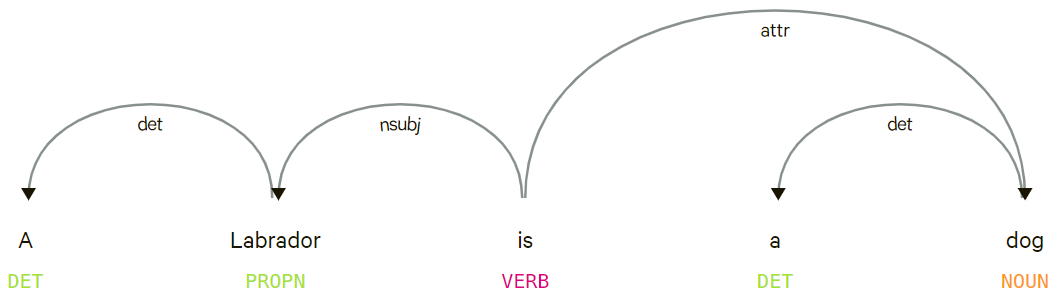
\includegraphics[width=1.\linewidth]{images/dependency_parse.png}
  \caption{Example dependency tree of a simple sentence.}%% \index{Dependency tree}}
  \label{fig:simple_dep_tree}
\end{figure}
The dependency path can be represented as a feature according to a bespoke notation.  An edge between two words can be captured with the tuple $(lemma, pos_tag, dependency_label, direction)$ and the link between two related words expressed as a list of edges.  The link between the hyponym \textit{Labrador} and its hypernym \textit{dog} would be expressed as the sequence:
\[(Labrador, PROPN, NSUB, <), (be, VERB, ROOT, -),(dog, NOUN, ATTR, >)\]

This particular notation is used in \citep{shwartz2016path} which we found more intuitive than the older convention used in \citep{Snow2004}.  To avoid longer, potentially less precise paths, a limit on the links between nouns can be imposed.  \citep{Snow2004} opted for the shortest path consisting of a maximum of four links between any two nouns.

To avoid extreme sparsity in the path vector model, \citeauthor{Snow2004} harvested dependency paths that held for at least five different word pairs from a corpus of 6 million news article sentences \citep{Snow2004}.  Doing so they generated 69,592 distinct dependency path features.  The corpus was also used to extract training and evaluation data.  As \citeauthor{wu2012probase} did later on in \citep{wu2012probase}, \citeauthor{Snow2004} extracted hyponym-hypernym word-pairs from each sentence in their corpus.  Invoking WordNet \citep{Miller1995} as lexical resource, they split the set of pairs into known hypernymy and random words.  To consider a word-pair, both of its constituent words had to be first detected in WordNet.  An ordered word-pair $(x, y)$ would be added to the known hypernym set, if $y$ is found to be an ancestor of $x$.  Words that were not hierarchically related were consigned to the random word list.  The ratio of known hypernyms to random words was 1:50.    

The dataset was used to evaluate the quality of the mined dependency paths.  This was done by applying a simple binary classifier to each path, and predicting hypernymy if a word-pair was connected by a dependency path at least once.  This exercise supplied quantitative support for the efficacy of Hearst’s manually derived patterns, all of which were found to be highly-predictive of hypernymy.  A further four patterns were also found to be high-performing:
\begin{itemize}
    \item $Y$ like $X$;
    \item $Y$ called $X$;
    \item $X$ is a $Y$;
    \item $X$, a $Y$;
\end{itemize}

\subsection{Leveraging Classifiers to Predict Hypernymy}
Intuitively, pattern occurrence frequency should be positively correlated to hypernym detection success.  \citeauthor{Snow2004} create two \ac{VSM}s.  One is a 69,592 dimensional matrix, where each dimension represents a particular dependency path and its value is the total number of times that dependency path connected an input word-pair.  They also create a bucketed, binary vector model where each dependency path corresponds to a 14-dimension “one-hot” encoded binary vector with each dimension capturing the number of pattern occurrences on an exponential scale from 1 (single occurrence) to 8192.  Thus, every word-pair is encoded as a 974,277-dimensional, sparse vector \citep{Snow2004}.  Using the same training set employed to quantify dependency path effectiveness, they train two logistic regression classifiers using each feature vector space respectively.  A significant improvement was observed compared to a simple Hearst pattern-only baseline, which classifies hypernymy if the presence of one or more Hearst patterns is found binding the input word-pair.  Their logistic regression model trained on the bucketed, “one-hot” vectors yields a 0.3480 F1 score, a 132\% improvement over the baseline \citep{Snow2004}. 
\citeauthor{ritter2009anyway}, on the other hand, advocate analysing the word form of the pattern-matched words, prior to proposing them as viable hypernym candidates \citep{ritter2009anyway}.  In particular, words detected in the plural-form by a POS-tagger are more likely to be precise hypernyms when found in certain in patterns \citep{ritter2009anyway}.  They also examine the importance of pattern occurrence frequency in their experiments, focusing on the standard Hearst patterns.  The ambiguity of the English language makes it such that high-frequency patterns alone cannot always guarantee correct hypernyms.  The authors furnish negative hypernymy examples, despite the matching highly-occurring patterns \citep{ritter2009anyway}:
\begin{itemize}
    \item \say{…all around the world including Australia, …} $\Rightarrow$ $hypernym(Australia, world)$
    \item \say{…information about this hotel such as rates, …} $\Rightarrow$ $hypernym(rates, hotel)$
    \item \say{My dog is a bloodhound} $\Rightarrow$ $hypernym(dog, bloodhound)$
\end{itemize}

They distinguish between “left” and “right” patterns where the hyponym $X$ features to the left or right of the hypernym $Y$ in a sentence.  The first two negative examples above are instances of “right” patterns and the last an incorrect instance of a “left” pattern.  \citeauthor{ritter2009anyway} engineer a set of frequency-related features for a given a word-pair.  In addition to total distinct pattern matches, they include features that capture “left” and “right” pattern matches; the total number of times that the hyponym is related to the hypernym via the lemma \textit{be}; the percentage of matches where the hyponym is preceded by an article, determiner or quantifier; the frequency rank of the hypernym with respect to the hyponym in the pair \citep{ritter2009anyway}.   

The word-pair dataset is extracted using \textsc{TextRunner} \citep{banko2007open}, applied on a 117 million web page corpus, which is then validated manually.  A test data-set consisting of 953 pairs is set aside and is split into common concepts (370 pairs) and named entities (583 pairs).  The pattern frequency vector is fed into \textsc{HypernymFinder$_{SVM}$}, a \ac{SVM} classifier \citep{platt1999probabilistic} designed to improve on an earlier na\"ive rules-based classifier that excluded hypernymy in word-pairs that did not match both left and right Hearts patterns.  An \ac{SVM} classifier splits the vector space by estimating hyperplanes which maximise the distance margin between them and the closest training-set samples.    
Unlike \citeauthor{Snow2004} who used WordNet as an evaluation and comparison tool \citep{Snow2004}, \citeauthor{ritter2009anyway} merge WordNet with \textsc{HypernymFinder$_{SVM}$} to create a hybrid classifier.  
Moreover, they opt for a hypernym discovery setup, foreshadowing the SemEval-2018 task 9 shared task \citep{camacho2018semeval}.  They retrofit the precision and recall metrics to measure respectively the percentage of overall correct hypermys and the percentage of terms for which one correct hypernym was proposed \citep{ritter2009anyway}.  

WordNet can return high-quality hypernyms but suffers from low coverage, especially with regards to named entities.  Each test candidate was first looked up in WordNet in which 17\% and 64\% of named entities and common nouns respectively were found.  Given some bounded vocabulary (details of which are elusive in their paper), the hybrid classifier outputs the five words it considers most likely to be hypernyms of the test words missing in WordNet.  In this manner, \citeauthor{ritter2009anyway} boosted the WordNet baseline for named entities and, to a lesser extent, common nouns.  Recall/precision increased from 0.17/1.0 to 0.32/0.9 and from 0.64/1.0 to 0.7/0.9 for named entities and common nouns respectively \citep{ritter2009anyway}.  Precision suffers with increased recall since the classifier’s output cannot be of the gold-standard level maintained in WordNet.

\subsection{Identifying Co-hyponyms to Increase Recall}
\citep{Snow2004} and \citep{ritter2009anyway} both acknowledge the limitation of Hearst patterns \citep{hearst1992automatic}.  Most hypernyms simply do not feature in the same sentence with their hyponyms \citep{Snow2004, ritter2009anyway}.  They hypothesise about extending the confines of the sentence for an “orphan” hyponym (i.e. no companion hypernym was found for it in a sentence) by finding co-hyponyms with known hypernyms.  If $(x_i, x_j)$ are two coordinate nouns and $hypernym(x_i, NA)$, $hypernym(x_j, y)$ then we can deduce $hypernym(x_i, y)$.

\citeauthor{Snow2004} experiment with various techniques including: building a distributional similarity vector space model; resorting to WordNet to find co-hyponyms for supported terms; and using high frequency conjunction dependency patterns.  Using the distributional similarity vector space the words can be scored for co-hyponym similarity using the symmetric cosine measure.  A linear combination of the probabilities calculated by the hypernym-only classifier and coordinate classifier increased the $F1$ score by 20\% compared to a hypernym-only classifier on a hand-labelled dataset ($F1$ of 0.3268 and 0.2714 respectively) \citep{Snow2004}.

On the other hand, \citeauthor{ritter2009anyway} were inspired by \textsc{Realm} \citep{downey2007sparse}, which uses \ac{HMM}s to perform type checking in an Information Extraction system, especially if the term in question is sparsely represented in vector space.  In \ac{HMM}s, a hidden stochastic process can only be glimpsed at through another stochastic process that produces a sequence of observations.  No information is known about the model's state but we can assume that there exists some model that can generate the data we're able to observe \citep{rabiner1989tutorial}.  For instance, \textit{Pickerington, Ohio} and \textit{Chicago, Illinois} are both cities but the former will be mentioned much less frequently in a balanced corpus.  Using traditional distributional similarity measures, it is unlikely that \textit{Pickerington} and \textit{Chicago} will be deemed similar since the contexts in which they appear are different.  However given an \ac{HMM} with $n$ hidden states that models the corpus, it is possible that $., Ohio$ and $., Illinois$ were generated by the same hidden states since both terms represent US States \citep{downey2007sparse} in \citep{ritter2009anyway}.

\citeauthor{ritter2009anyway} applied the same concept to finding terms similar to a given hyponym.  To do so, a word is represented by the distribution of the hidden states’ probability of the term being generated by the \ac{HMM} model.  Thus, given an \ac{HMM} model with $n$ states, an $n$-dimensional vector representation is returned.  Similar words to a given term were found by applying a similarity metric on the \ac{HMM}-based feature vector.  The final incarnation of the authors' hypernym finder, is a linear combination of the probability calculated by the \textsc{HypernymFinder$_{SVM}$} classifier and the probability that a given term $x$ has a coordinate word which is a hyponym of the candidate hypernym $y$. Since word similarity alone is tenuous evidence for such words sharing a hypernym, the \ac{HMM} classifier predicts hypernymy in a $(x, y)$ word-pair only if $x'$ exceeds a similarity threshold with $x$, and $x'$ is hyponym of $y$ \citep{ritter2009anyway}.

\subsection{Encoding Dependency Paths with an LSTM} \label{HypeNet}
We have seen that using dependency paths as features can lead to a highly-dimensional vector space.  In one study we have examined, almost 70,000 distinct dependency paths were extracted from a corpus.  Vectors will be sparse since a particular word-pair will only activate a small number of dependency paths.  To improve dependency path representation, \citeauthor{shwartz2016path} trained a \ac{LSTM} \citep{hochreiter1997long} encoder to learn path vectors that are optimised towards detecting hypernymy \citep{shwartz2016path}.  The path vectors are fed into a classifier which predicts whether the dependency pattern feature captures the hypernymy relationship in a given word-pair.  The model is referred to as \textsc{HypeNET} \citep{shwartz2016path}.

The LSTM belong to a family of neural models known as \ac{RNN}s.  Contrary to regular densely-connected networks which require an entire sequence to be presented at once, \ac{RNN}s can be fed the input, one time-step at a time \citep{chollet2017deep}.  A limitation of \ac{RNN}s is their difficulty to recognise signals that come from distant points in a past sequence which does not make them the ideal choice to learn long-term dependencies.  The \ac{LSTM} overcomes this problem because it is a type of recurrent neural network with the ability to learn long-term dependencies.  By having access to the previous time-steps, it is able to build temporal patterns.  Through the use of a special gate composed of a dot product operator and activation function, it can selectively “forget” irrelevant signals whilst retaining information that is more important at the current time-step \citep{chollet2017deep}.  

The motivation behind using the \ac{LSTM} approach is to generalise the lexical-semantic relation between terms that holds in a multitude of contexts.  Prior to feeding them to the \ac{LSTM}, each word-pair is represented by a sequence of dependency paths in which the words co-occur in the corpus.  To be considered, a word-pair needs to co-occur in the corpus and be represented by at least two unique dependency paths.  The path is represented by a list of edge vectors with each edge made up of the concatenation of the embeddings of the lemma, \ac{POS} tag, dependency label and direction.  The dimensionality of the embeddings vary: \citeauthor{shwartz2016path} use 50, 4, 5, and 1 dimension for each respective component \citep{shwartz2016path} although this is not set in stone.  Hyper-parameter tuning on a validation set can help determine the best network configuration.  The \ac{LSTM} should learn which dependency path sequences are predictive of hypernymy while conveniently forgetting those which have no consequence on the semantic relationship \citep{shwartz2016path}.

The weighted-average of the encoded dependency path vectors is computed prior to feeding it to a softmax classifier, trained to minimise cross entropy loss.  The softmax classifier assigns a probability for both the hypernymy and non-hypernymy target labels, which sum up to 1.

\citeauthor{shwartz2016path} compare their novel approach to \citeauthor{Snow2004}'s model \citep{Snow2004} we discussed in section \ref{Learning Patterns Automatically}. The authors train a logistic regression classifier on the 100,000 most information paths chosen using chi-squared feature selection.  On a random data split, the sparse model returns a precision of 0.843 compared to \textsc{HypeNET}’s 0.811 but the latter scores 0.716 recall, a 58\% improvement over \citeauthor{Snow2004}'s model.    

\section{Distributional Model Overview}
%% Need to find out how to type-set Maltese unicode characters
\say{Ghidli ma’ min taghmilha, u nghidlek x’int} is a Maltese expression which means that the company a person keeps says a lot about that person.  The linguist J.M. Firth (1957) cast a similar sentiment to words, saying that a word’s neighbours can divulge much about that word.  This dictum is framed by the Distributional Hypothesis \citep{harris1954distributional} which states that words with similar meaning occur in similar contexts.  

The Distributional Hypothesis is encapsulated in a \ac{VSM} (also referred to as distributional model), a matrix-type data structure which, at its simplest, captures the occurrences of \textit{row} events in \textit{column} contexts. The matrix’s structure in terms of what the rows and columns represent is a design decision and depends on the statistical semantic hypothesis the matrix is supposed to model.  We will briefly discuss the word-context and pair-pattern matrices, the two main types featured in the hypernymy discovery literature.  We also mention the term-document matrix, which we did not encounter in the literature review but which preceded the other two data structures and influenced their development.  The term-context feature is found at the intersection of row and column.  Features can either be expressed as raw frequencies (positive integers including 0) or can be mapped by a weighting function.  In the latter case the frequency value will be a real number.

The objective of a vector space model \ac{VSM} is to convert discrete word symbols into points in higher-dimensional space \citep{turney2010frequency}.  The word symbol does not convey any meaning through its surface form; however, by projecting each word to a multi-dimensional vector, points that are close according to some distance metric will exhibit some form of semantic relatedness.  Conversely, words corresponding to points that are far apart will tend to be weakly related or entirely unrelated \citep{turney2010frequency}.

We will discuss the matrix types in the following section.  We shall borrow the mathematical notation used in \citep{turney2010frequency} as follows:
\begin{itemize}
    \item $\textbf{X}$ will be our matrix which will be made up of $m$ rows and $n$ columns;
    \item $\textbf{X} \in \mathbb{N}^{m \times n}$ if the frequency is unweighted or $\textbf{X} \in \mathbb{R}^{m \times n}$ if we are adopting a frequency weighting mechanism;
    \item $\textbf{x}_{i:}$ will be a row-vector of $n$ elements representing a word $w_i$ in a vocabulary of terms, extracted from a corpus;
    \item $\textbf{x}_{:j}$ will be a column-vector of $m$ elements representing a document, context or pattern depending on the matrix type;
    \item $x_{ij}$ is a scalar value and measures the association between target word $w_i$ and context/pattern/document $c_j$
\end{itemize}    

Most of the elements of $\textbf{X}$ will be set to zero since a word cannot appear in all contexts and each context will correspond to a small percentage of the entire vocabulary.  Such a matrix is referred to as a sparse matrix, which contrasts with a dense matrix which has non-zero values in most of its elements.

\subsection{Mapping Vector Space Models to Semantic Hypotheses}
Word patterns can be statistically examined to understand how humans attribute meaning to the words \citep{turney2010frequency}.  Four main hypotheses were developed, supported by a corresponding mathematical matrix structure that allows each hypothesis to be explored empirically.

\subsubsection{Bag of Words}
According to the bag of words hypothesis \citep{salton1975vector}, we can represent a document in terms of the frequency distribution of the words that compose it.  The term-document matrix is the ideal structure to model this hypothesis.  X will be composed of a vocabulary of m words, extracted from n documents where each row $\textbf{x}_{i:}$ vector is a term word and each column vector $\textbf{x}_{:j}$ is a document.  Thus, the document is represented as a bag of words vector, where each dimension contains the frequency of a word $w_i$ in the document.  In the bag of words model, several aspects of language use are lost, including sequential word ordering, and syntactic links between the words.  Indeed the entirety of the document structure is absent since we cannot tell how the words were strung together in sentences, paragraphs and sections.    Despite these misgivings, the bag of words technique can effectively capture similarity between documents on the basis of word distribution alone \citep{turney2010frequency}.  This result is supported by the intuition that the domain or topic of a document influences the choice of the words used to compose the document \citep{turney2010frequency}.

\subsubsection{Word-context}
The term-document matrix may be an effective tool to measure document similarity or retrieve the most relevant documents to a given query.  However, a document is far too wide to make an ideal context if we are interested in word similarity.  The distribution hypothesis is better served by a word-context matrix.  \citep{lund1996producing} in \citep{turney2010frequency} proposed a window-based context which only considers a number of words before and after a target word.  The $k$ surrounding words of target word $w$ are: $w-k, \ldots, w-1, w+1, \ldots, w+k $.  

The typical context window size is fairly small, consisting of two to five words \citep{roller2014inclusive, santus2014chasing, shwartz2017siege}.  However, wider context windows are also acceptable.  For instance, in \citep{roller2014inclusive}, one of the context windows spanned an entire corpus sentence.

The context windows can be optionally decorated with their direction with respect to a target word \citep{shwartz2017siege}.  In the sentence \textit{The quick brown fox jumped over the lazy dog}, the directional context of the target word $fox$ is $(quick^-, brown^-, jumped^+, over^+)$. In a non-directional window, the left and right context words are indistinguishable.   

Contexts are not necessarily limited to adjacent words; \citep{lin1998information} in \citep{turney2010frequency} and \citep{levy2014dependency} employed dependency-based contexts.  To build their experimental distributional semantic spaces, \citep{shwartz2017siege} considers both parent-daughter and parent-sister neighbours in a dependency tree.

\subsubsection{Pair-pattern}
The term, represented in the matrix row, is no longer a single word but a word-pair and the matrix column feature becomes a doubly-linked pattern which ties the term word-pair together.  We have seen a pair-pattern matrix in action in \citep{Snow2004}.  The term pair is a tuple containing a hyponym and a candidate hypernym.  Tuples can be positive or negative pairs depending on whether the candidate word is an actual hypernym.  The matrix column feature was a dependency path which linked the two words together by the concatenation of edge links in the parse tree and the feature value was the frequency a word-pair matched that particular pattern.

\citep{lin2001discovery} quoted in \citep{turney2010frequency}, propose the extended distributional hypothesis which states that patterns fitting similar pairs tend to have the same semantics.  Conversely, the latent relation hypothesis states that word pairs captured by similar patterns tend to be bound by a similar semantic relation \citep{turney2010frequency}.  \citep{Snow2004} opted for a supervised approach and utilised various classifiers to learn which paths were mostly indicative of hypernymy.  The path feature set they induced included any path that linked at least five distinct nouns pairs extracted from each sentence in the corpus.  

A variant of the pair-pattern matrix is \textbf{TypeDM} \citep{roller2014inclusive}, where a matrix row represents a term word and the context column is a pair consisting of a context word and a syntagmatic relationship that ties the two words together.

\subsection{Feature Weighting}
At its most elemental, each matrix type quantifies the association between a context and a term by counting the occurrences of the term in a particular context \citep{turney2010frequency}, \citep{shwartz2017siege}.  Often, the raw frequencies are adjusted to compensate for the fact that some words convey little information despite their high recurrence in a corpus.  In the bag of words model, the raw frequencies are transformed using the \textbf{\ac{tf-idf}} function family \citep{turney2010frequency}.  This compels a term to score a high weight if its presence in a document is proportional to its scarcity in other documents.

An alternative to \ac{tf-idf} used to weight features in a word-context matrix is \ac{PMI}:
\[PMI(w_i, c_j) = log \Bigg( \frac{p(w_i, c_j)}{p(w_i)p(c_j)} \Bigg) \]
\ac{PMI} measures the log ratio of the joint probability of a word $w_i$ in a context $c_j$ and the product of the marginal probabilities of $w_i$ and $c_j$ \citep{church1990word} in \citep{turney2010frequency, shwartz2017siege}.

If there is an interesting relationship between $w_i$ and $c_j$, then the conditional probability of $w_i$ given $c_j$ is greater than the joint probability of $w_i$ and $c_j$ given that the two are mutually exclusive.  When that is the case, \ac{PMI} returns a positive value.  On the other hand, if $w_i$ and $c_j$ are independent, \ac{PMI} returns a zero value.  If the presence of a particular context decreases the probability of a word co-occurring, then $p(w_i, c_j)$ is smaller than $p(w_i)p(w_j)$ and a negative \ac{PMI} is returned.

A variant of \ac{PMI} is \ac{PPMI} which enforces every matrix element to be positive or zero if a word does not occur in a particular context.  \ac{PPMI} is biased towards rare events \citep{turney2010frequency} but this can be neutralised by the application of \ac{PLMI} which is returned when \ac{PPMI} is multiplied by the co-occurrence frequency of $w_i$ and $c_j$ \citep{evert2008corpora} in \citep{shwartz2017siege}.

\subsection{Building a Vector Space Model}
A pre-processing pipeline is applied to a corpus before it can be transformed into a matrix-based mathematical model.  The pipeline includes tokenisation, normalisation and, optionally, annotation steps \citep{turney2010frequency}.

At first glance, tokenisation of an English corpus may seem like a trivial task since words are conveniently separated by spaces and sentences divided by the full-stop punctuation mark.  A tokeniser must, however, contend with specificities such as hyphenated words, abbreviations, diverse use of punctuation (ex. \textit{can’t}, \textit{isn’t}, etc.) and multi-word phrases that should be treated atomically (ex. \textit{catch fire}, \textit{vice president}, \textit{Daniel Day-Lewis}) .  Pictogram-based languages such as Chinese and Japanese are harder to deal with since words are not separated by spaces to begin with \citep{turney2010frequency}.

Words expressed with different lexicalisations can sometimes have the same meaning.  A chief example is the capitalisation of a word at the beginning of a sentence which does not change the meaning of the word. Normalisation smoothens surface form variation by lower casing and stemming words. Stemming reduces a word to its most generic form which may not be an actual word.  Highly specific word forms can harm recall which is thus augmented by normalisation but only at the expense of precision \citep{kraaij1996viewing} in \citep{turney2010frequency}.

Annotation increases the specificity of a word by decorating it with descriptors such as the part-of-speech tag, word sense tag, and dependency parse labels.  Word sense disambiguation is particularly relevant in the field of hypernymy detection and discovery since disparate meaning is often attributed to identical word forms.  The hypernym of \textit{bank} can either be \textit{incline} or \textit{financial institution} depending on its word sense.  The attachment of more information to a word is expected to increase precision while punishing recall \citep{turney2010frequency}.

We briefly mentioned all the components needed to build a \ac{VSM} from pre-processing to feature weighting.  To find the degree to which $y$ is a hypernym of $x$ in word-pair $(x, y)$, a metric is applied to the vector representation of $x$ and $y$.  The metrics are collectively referred to as unsupervised methods since they are applied without the need of training data.  In the following section we explore unsupervised methods within selected literature.

\section{Unsupervised Methods}
\subsection{Metric Overview}
Unsupervised methods consists of metrics grouped into four categories, each representative of a hypernymy inflected semantic hypothesis.  \citeauthor{shwartz2017siege} furnish us with an exhaustive survey of metrics across all categories which are listed below.  In all descriptions, $\textbf{x}$ and $\textbf{y}$ represent the term word (hyponym) and candidate hypernym feature vector respectively.  A summary of unsupervised measures which can be used to estimate hypernymy simalarity can be seen in Table~\ref{tab:unsupervised_measures}.

%% Table summarising the measures and grouping them by hypothesis needs to come here
\renewcommand{\arraystretch}{1.2} 
\begin{table*}\centering
    \begin{tabular}{@{}ll@{}} \toprule
    \textbf{Metric}              & \textbf{Source} \\ 
    \cmidrule{1-2}
    \multicolumn{2}{c}{Similarity Measures} \\ \cmidrule(lr){1-2}
    $Cosine Similarity$   & \citep{salton1975vector} \\
    $Lin Similarity$      & \citep{lin1998information} \\
    $APSyn$               & \citep{santus2016unsupervised} \\
    \cmidrule{1-2}
    \multicolumn{2}{c}{Inclusional Measures} \\ \cmidrule(lr){1-2}
    $Weeds Precision$     & \citep{weeds2003general} \\
    $cosWeeds$            & \citep{lenci2012identifying} \\ 
    $ClarkeDE$            & \citep{clarke2009context} \\
    $balAPinc$            & \citep{kotlerman2010directional} \\
    $invCL$               & \citep{lenci2012identifying} \\
    \cmidrule{1-2}
    \multicolumn{2}{c}{Informativeness Measures} \\ \cmidrule(lr){1-2}
    $SLQS$                & \citep{santus2014chasing} \\
    $SLQS_{Sub}$            & \citep{shwartz2017siege} \\
    $SLQS_{Row}$            & \citep{shwartz2017siege} \\
    \cmidrule{1-2}
    \multicolumn{2}{c}{Reversed Inclusional Measures} \\ \cmidrule(lr){1-2}
    $Reversed Weeds$      & \citep{shwartz2017siege} \\
    $Reversed ClarkeDE$   & \citep{shwartz2017siege} \\
    \bottomrule
    \end{tabular}
    \caption{Unsupervised Hypernymy Similarity Measures.}\label{tab:unsupervised_measures}
\end{table*}


\subsubsection{Similarity Measures}
Following the distributional hypothesis \citep{harris1954distributional}, similarity measures focus on the symmetric similarities between the hyponym and hypernym.  Cosine similarity is the inner product of the unit-normalised vectors $\textbf{x}$ and $\textbf{y}$, thus placing the onus of similarity on the angle between the vectors.   The cosine metric measures word similarity by the angle between the vectors $\textbf{x}$ and $\textbf{y}$ where acute angles indicate higher similarity.  The Lin measure is the ratio between common contexts and separate contexts of $\textbf{x}$ and $\textbf{y}$.  $APSyn$ is a symmetric measure that computes the extent of intersection among the $N$ most related contexts of two words, weighted according to the rank of the shared contexts ($N$ is a hyper-parameter) \citep{santus2016unsupervised}.

\subsubsection{Distributional Inclusional Measures}
A common criticism of the measures based on the distribution hypothesis is that they are not able to discern among various semantic relations \citep{roller2014inclusive}.  A term word’s nearest neighbours will bear some semantic relationship to it but is not guaranteed to be its hypernym. Moreover, the distributional hypothesis fails to acknowledge the asymmetric nature of hypernymy.  Instead, this is better captured by the distributional inclusional hypothesis \citep{geffet2005distributional} which states that the main contexts of the hyponym term are absorbed in the contexts of its hypernym.  According to this hypothesis, plugging in the generic term instead of the specific term in a sentence would not warp the sentence’s meaning.  $Weeds Precision$ \citep{weeds2003general} is an example of an asymmetric metric that computes the weighted inclusion of the contexts of $\textbf{x}$ within the contexts of $textbf{y}$.  Details of the other measures may be found in their respective papers.

$invCL$ \citep{lenci2012identifying} is another example of an inclusional metric which is calculated as the geometric mean of the degree of inclusion of the hyponym’s contexts in the hypernym’s contexts  and the non-inclusion of the hypernym’s contexts into the hyponym’s contexts.


\subsubsection{Distributional Informativeness Measures}
\citeauthor{santus2014chasing} debated the validity of the distributional inclusional hypothesis.  They argue that the distinction between a hyponym and a hypernym lies in the generality of their contexts.  By virtue of their abstract qualities, hypernyms occur in broad contexts.  Their hyponyms, on the other hand, are specific and thus more likely to feature in explicit contexts.  For instance, an animal has general properties of locomotion, feeding and reproduction but only the echidna and platypus will feature in the context of egg-laying mammals.

The distributional informativeness hypothesis is derived from this principal.  $SLQS$ \citep{santus2014chasing} employs entropy to quantify informativeness.  Lower entropy values imply less uncertainty about the outcome of an event.  Hence, the more general the contexts, the lower the probability we can guess the “topic” of reference and the higher the entropy value.  $SLQS$ calculates the reciprocal difference of the median entropy of the top $N$ contexts of hyponym and hypernym vectors.  $SLQS$ is also an asymmetric measure and if $SLQS(x, y)$ yields a positive value, then $\textbf{y}$ is found to be more general than $\textbf{x}$ which is an indicator of hypernymy.  Three further variants of $SLQS$ were first proposed in \citep{shwartz2017siege}.  $SLQS_{Sub}$ is a weakly symmetric version of $SLQS$ evaluated by subtracting the median entropy of a hyponym's top $N$ contexts from the median entropy of its hypernym's top $N$ contexts.  $SLQS_{Row}$ exploits the fact that the context and target word entropies are not highly correlated, thus repositioning $SLQS$ in terms of target word entropy \citep{shwartz2017siege}.  Finally, $SLQS_{Row, Sub}$ uses the same subtraction expression as $SLQS_{Sub}$ on $SLQS_{Row}$.

\subsubsection{Reversed Inclusional Measures}
The distributional inclusional hypothesis is directly challenged by the reversed inclusional measures.  The basis of these measures is the hypernym cannot always replace the hyponym in its contexts due to the high specificity of the latter.  \textit{The mammal climbed into the car} would not be a reasonable alternative for \textit{the man climbed into car} despite the fact that a man is a mammal.  \citep{shwartz2017siege} propose a simple variant of Weeds Precision and ClarkeDE to model this property, consisting of switching the original function parameters around.  Thus $WeedsPrec(x,y)$ becomes $ReversedWeedsPrec(y, x)$ and the same principle applies to ClarkeDE.

\subsection{Application of Unsupervised Metrics in Selected Literature} \label{shwartz_unsupervised}
In \citep{santus2014chasing},  a 2.7-billion word corpus was constructed by concatenating the ukWaC \citep{ferraresi2007building} and WaCkypedia corpora in English \citep{baroni2009wacky}.  Word context was provided by a two-word window on either side of the target word and \ac{LMI} was used to weight the features.  The BLESS dataset \citep{Baroni2011} was recruited as an evaluation dataset.  Besides providing hypernyms for 200 English concepts, BLESS also features several negative examples of hypernymy which include other semantic relations such meronym, co-hyponymy and randomly unrelated words.

\citeauthor{santus2014chasing} pitted the distributional inclusional and informativeness hypotheses against each other over two tasks.  $WeedsPrec$ \citep{weeds2003general} represents the inclusional metric family while the informativeness hypothesis is represented by $SLQS$ \citep{santus2014chasing}.  The first tasks involves detecting hypernymy in each positive word-pair using the most frequently occurring word as a baseline.  The second, harder task consisted of discriminating hypernymy from the other semantic relations.

\begin{table*}\centering
    \begin{tabular}{@{}lrrrr@{}} \toprule
    \textbf{Metric}  & \textbf{Hypernymy} & \textbf{Co-hyponymy} & \textbf{Meronymy} & \textbf{Unrelated} \\
    \cmidrule{1-5}
    \textit{Baseline}   & $0.40$ & $0.51$ & $0.38$ & $0.17$ \\
    \textit{Cosine}   & $0.48$ & $0.46$ & $0.31$ & $0.21$ \\
    \textit{WeedsPrec}   & $0.50$ & $0.35$ & $0.39$ & $0.21$ \\
    \textit{SLQS $\times$ Cosine}   & $\textbf{0.59}$ & $\textbf{0.27}$ & $\textbf{0.35}$ & $\textbf{0.24}$ \\
    \bottomrule
    \end{tabular}
    \caption{Average precision of two unsupervised metrics when discriminating semantic relations.}\label{tab:santus_comparison}
\end{table*}

$WeedsPrec$ does not beat the baseline in the first task, scoring a precision of $0.6304$ (compared to a $0.6609$ baseline) while $SLQS$ does better, yielding a precision score of $0.87$.  Distributional similarity is leveraged in the second task by assuming that a hypernym observes two rules: the hyponym must be distributionally similar to the hypernym; the hypernym must be more general than the hyponym.  To merge the two, the product of cosine similarity and positive $SLQS$ is computed.  Precision is replaced by \ac{AP} as evaluation metric where \ac{AP} evaluates the ranking of the predicted hypernymy word-pairs against false positives pertaining to other relations.  The results are reproduced in Table~\ref{tab:santus_comparison} from \citet{santus2014chasing}.

$SLQS$ is less likely to confuse co-hyponymy for hypernymy than $WeedsPrec$ which suggests that in general the co-hyponym in the candidate word slot ($y$) is as specific as the query word ($x$).  The scores reflect the average precision over all 200 concepts in the BLESS dataset ($AP@all$).

In \citep{shwartz2017siege}, the authors undertake a more ambitious study of unsupervised metrics over four commonly-used datasets: BLESS \citep{Baroni2011}; EVALution \citep{santus2015evalution}; Lenci/Benotto \citep{benotto2015distributional}; and Weeds \citep{weeds2014learning}.  Each dataset features positive hypernymy examples and negative examples consisting of words that are related together via some other semantic relationship such as meronymy, synonymy, co-hyponymy or randomly unrelated.  The study tests each metric’s ability at distinguishing hypernymy from the other relations.  Furthermore, experiments were also carried out to measure the metric’s performance at detecting hypernymy among specific relations in isolation. 

\begin{table*}\centering
    \begin{tabular}{@{}cccc@{}} \toprule
    \textbf{Context Type} & \multicolumn{2}{c}{\textbf{Context Parameters}} & \textbf{Feature Weighting} \\ \cmidrule{1-4}
    \multirow{6}{*}{Window} & 
    \multirow{3}{*}{Directional} &
    \multirow{3}{*}{$win2d$ or $win5d$} & Raw Freq \\
    & & & PPMI \\
    & & & LMI \\ 
    \cmidrule{2-4}
    & \multirow{3}{*}{Non-Directional} &
      \multirow{3}{*}{$win2$ or $win5$} & Raw Freq \\
    & & & PPMI \\
    & & & LMI \\ 
    \cmidrule{1-4}
    \multirow{3}{*}{Dependency} & 
    \multirow{3}{*}{-} &
    \multirow{3}{*}{$dep$ or $joint$} & Raw Freq \\
    & & & PPMI \\
    & & & LMI \\
    \bottomrule
    \end{tabular}
    \caption{Vector Space Model combinations used in \citep{shwartz2017siege}.}\label{tab:siege_vector_spaces}
\end{table*}

Following \citep{santus2014chasing}, \citeauthor{shwartz2017siege} make use of the same concatenated corpus but in contrast to \citeauthor{santus2014chasing}, lemmatised it and annotated it with part-of-speech tags and dependency labels.  The \ac{VSM}’s vocabulary was limited by only considering nouns, verbs and adjectives that featured 100 times or more in the corpus.  Several \acl{VSM}s were constructed in an attempt to determine which particular combination, in tandem with an unsupervised metric, works best at identifying hypernymy among several relata.  

Table~\ref{tab:siege_vector_spaces} illustrates the \ac{VSM} variants tested.  The authors tested window and dependency contexts, with the association between the words and their contexts weighted by raw frequency, \ac{PPMI}, and \ac{PLMI} for a total of 18 matrix combinations. $win2$ and $win5$ represent a two and five word non-directional context window respectively, whereas the $d$ suffix denotes a directional context.  The dependency-based contexts are denoted by $dep$ and $joint$, where the former represents parent-daughter context and the latter captures parent-sister pairs in the dependency tree.

\begin{table*}\centering
    \begin{tabular}{@{}lccccr@{}} \toprule
    \textbf{Dataset} & \shortstack{\textbf{Hyper vs.} \\ \textbf{Relation} } & \textbf{Measure} & \shortstack{\textbf{Context} \\ \textbf{Type} } & \shortstack{\textbf{Feature} \\ \textbf{Weighting}} & \textbf{AP@100} \\ \cmidrule{1-6}
    \multirow{5}{*}{EVALution} & 
    All Relations & $invCL$ & joint & freq & 0.661 \\
    & Meronym & $APSyn$ & joint & freq & 0.883 \\
    & Attribute & $APSyn$ & joint & freq & 0.880 \\
    & Antonym & $SLQS_{Row}$ & joint & freq & 0.740 \\
    & Synonym & $SLQS_{Row}$ & joint & freq & 0.830 \\
    \cmidrule{1-6}
    \multirow{5}{*}{BLESS} & 
    All Relations & $invCL$ & win5 & freq & 0.540 \\
    & Meronym & $SLQS_{Sub}$ & win5d & freq & 1.000 \\
    & Coordinate & $SLQS_{Sub}$ & joint & freq & 0.995 \\
    & Attribute & $SLQS_{Sub}$ & dep & PLMI & 1.000 \\
    & Event & $APSyn$ & dep & freq & 1.000 \\
    \cmidrule{1-6}
    \multirow{3}{*}{Lenci/Benotto} & 
    All Relations & $APSyn$ & joint & freq & 0.617 \\
    & Antonym & $APSyn$ & dep & freq & 0.861 \\
    & Synonym & $SLQS_{Row, Sub}$ & joint & PPMI & 0.948 \\
    \cmidrule{1-6}
    \multirow{2}{*}{Weeds} & 
    All Relations & $ClarkeDE$ & win5d & freq & 0.911 \\
    & Coordinate & $ClarkeDE$ & win5d & freq & 0.911 \\
    \bottomrule
    \end{tabular}
    \caption{Subset of best unsupervised results in \citep{shwartz2017siege}.}\label{tab:siege_unsupervised_results}
\end{table*}

For each measure, context-type, feature weighting function, the word-pairs were ranked in descending order of the score achieved.  The \ac{AP} was measured in two instances: on the full list of word-pairs; and on the 100 most confidently scored pairs.  A table reflecting the best $AP@100$ results recorded in the experiments is shown in Table~\ref{tab:siege_unsupervised_results} from \citet{shwartz2017siege}.

Results suggest that there does not exist one combination of measure and semantic space that outperforms the rest across the board.  Supported by the best results, the authors speculated that syntactic contexts (dependency, joint-dependency) have higher hypernymy predictive power due to them capturing both proximity and syntactic features.  The na\"ve raw frequency feature weight acquitted itself surprisingly well considering it does not provide more information than co-occurrence of word and context.

The nature of the word-pairs in the datasets influenced the experiments’ outcome and shed some light on why some metrics fared better on some datasets than others.  $SLQS$ outputs a high score if the candidate word being tested for hypernymy is found to be more general than the query word \citep{santus2014chasing}.  It performed well (although not necessarily the best) in the hypernymy/antonymy, hypernymy/synonymy challenges where the (negative) candidate antonyms and synonyms were largely less general than the hypernyms in the set.  Conversely, the symmetric similarity measures were best suited to distinguish hypernymy from words which have few shared contexts.  For instance, the attribute words featured in BLESS are adjectives which share few contexts with the noun term word.  

Like \citep{santus2014chasing}, $SLQS$ was more effective at recognising hypernymy than inclusion-based methods, even when applied onto dependency-based context types.  However, inclusion-based methods such as $ClarkeDE$, $invCL$ and $WeedsPrec$ were superior to $SLQS$ on the Weeds dataset.  \citeauthor{shwartz2017siege} conclude that this result is due to the distribution of words in Weeds, in which every positive and negative hypernym instance features only once.  BLESS contains several repeated hypernyms which, moreover, tend to be rather general (ex. \textit{animal}, \textit{object}).  This plays to the strengths of $SLQS$ which justifies its dominance on this particular set.

\subsection{Criticism of Unsupervised Methods}
We examined empirical work which illustrated the power of unsupervised metrics, founded as they are on sound linguistic hypotheses.  Although the metrics have been used in a hypernymy detection context, they can be leveraged to discover hypernyms by finding the nearest neighbours of a hyponym vector in a particular vector space according to an asymmetric measure based on the distributional inclusional or informativeness hypothesis like the baselines created by the SemEval-2018 Task 9 organisers \citep{camacho2018semeval}.  For unsupervised methods to be effective in this regard, the score returned when considering a hypernymy word-pair must be statistically distinguishable from the score returned if the word-pair is random or linked by some other semantic relation.  Otherwise recognising hypernyms using such methods is reduced to a game of chance.  Although \citep{santus2014chasing} challenged the soundness of inclusion measures, \citep{roller2014inclusive} tested whether asymmetric metrics based on the inclusional hypothesis are able to fulfill this requirement and, unfortunately, found them initially lacking.

\citeauthor{roller2014inclusive} construct a corpus in a manner similar to \citep{santus2014chasing}, but enlarged by the inclusion of Gigaword and BNC.  The authors pre-processed the corpus by lemmatising it and annotating the part-of-speech tags, after which they filtered out words which occurred less than 500 times.  They constructed three vector spaces, two of which were based on a window context (2 words around the target word, and a full sentence respectively), and one based on a TypeDM tensor model.  The vector spaces are denoted as \textit{U+W2}, \textit{U+Sent} and \textit{TypeDM} respectively.  The features of the two window-based models were transformed by \ac{PPMI}.

\begin{figure}[ht!] 
  \centering
  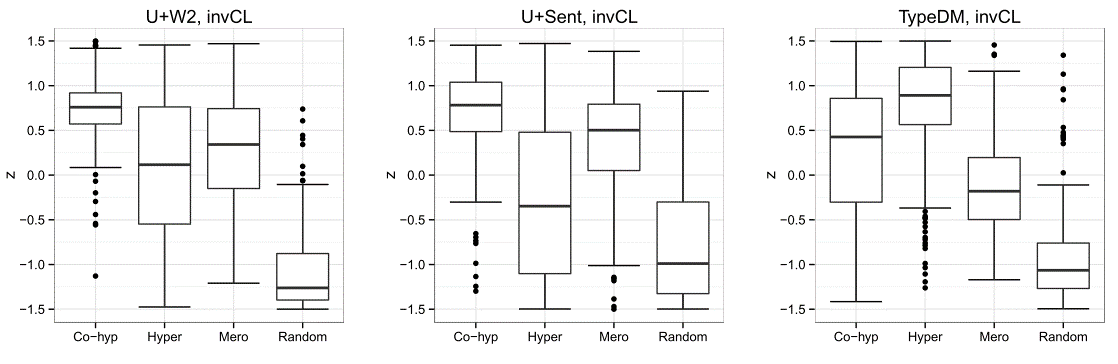
\includegraphics[width=1.\linewidth]{images/standardised_distribution_invCL.png}
  \caption{Standardised distribution of $invCL$ score in \citep{roller2014inclusive}.}
  \label{fig:standardised_invCL_boxplot}
\end{figure}

A battery of inclusional measures, including $WeedsPrec$ \citep{weeds2003general} and $invCL$ \citep{lenci2012identifying}, were used to score the word-pairs in the BLESS dataset \citep{Baroni2011} in each vector space which, as we have already seen, consists of word-pairs tied by several semantic relations.  The scores were standardised and a box-plot of the score achieved when measuring $invCL$ asymmetric similarity - chosen for the best results attained in the experiment - across relations and vector spaces is reproduced in Figure~\ref{fig:standardised_invCL_boxplot} from \citet{roller2014inclusive}.

Despite $invCL$ was the most productive metric at hypernym identification, we can see that performance is not robust across all vector space models.  The standardised $z$-score was significantly higher for hypernymy word-pairs in the \textit{TypeDM} space but was entirely deprived of predictive ability in the \textit{U+W2}  and \textit{U+Sent} \ac{VSM}s. \ac{AP} results for hypernymy against co-hyponymy, meronymy and random relation respectively, depict a similar picture.  In all vector spaces except \textit{TypeDM}, both the asymmetric measures as well as the baseline cosine symmetric measures assigned the highest ranking to co-hyponym terms by a significant margin.  In \textit{TypeDM}, $invCL$ acquires a higher mean average precision for hypernyms than for co-hyponyms but the difference is not statistically significant \citep{roller2014inclusive}.

These experiments pose a conundrum for unsupervised methods research: they have been shown to be successful in some settings but clearly miss the mark in others.  \citeauthor{roller2014inclusive} argued that the distributional inclusional hypothesis was selective and did not apply on all contexts.  However, unsupervised methods of distributional inclusion considered all contexts equally, which ultimately harms their performance \citep{roller2014inclusive}.  They propose a technique similar to \citep{Snow2004}, which leverages a supervised classifier to both learn the distributional signals most associated with a given set of hypernymy word-pairs, and interpret the trained models to understand which features are contributing to the estimated result.

\section{Supervised Methods}
High-quality, ground-truth data and associated target discrete labels (or continuous values if the task is of the regression type), distinguish supervised methods from the unsupervised measures we have reviewed so far.  In the hypernymy identification domain, supervised methods are not grounded in a linguistic hypothesis but attempt to learn the asymmetric metric from a provided training set \citep{levy2015supervised}.

Just like in the unsupervised context, the query and candidate hypernym terms are represented by vectors sourced from a vector space model.  Instead of applying distributional hypotheses, the vectors representing the words in the pair are combined by a vector operations like concatenation \citep{baroni2012entailment}, or difference \citep{roller2014inclusive}.  In the concatenation case, the hypernym vector is added to the tail of the hyponym vector to create a feature which has twice the number of dimensions as the individual word vector.  In the diff case, the hypernym vector is subtracted from the hyponym \citep{roller2014inclusive} or vice versa \citep{shwartz2017siege}.  The combined feature vectors are fed into a classifier together with the target labels.  The literature we reviewed shows a preference for the logistic regression \citep{roller2014inclusive, shwartz2017siege, levy2015supervised, yamane2016distributional, bernier2018crim} and \ac{SVM} classifiers \citep{shwartz2017siege, levy2015supervised, baroni2012entailment}.

\subsection{Classifier Background}
\subsubsection{Logistic Regression}
Despite the name, logistic regression is actually a binary classification learning algorithm that uses the properties of the logistic function $\sigma(z)=\frac{1}{1 + e^{-z}}$ that maps real valued inputs to values between $0$ and $1$.  Values in this range can be interpreted as a probability. The real value input is a linear combination of $m$ features and $m+1$ weights.  This can be expressed in the terms of the logit function: \[logit(p(y = 1 \mid x)) = z = \textbf{w}^T\textbf{x}\]

The resulting real value can be mapped to a probability using the defined logistic equation.  To learn the best weights (or coefficients) a cost function is required to minimise the error when predicting hypernymy.  This is done by minimising the logistic loss function, where $y$ in this case represents the target class rather than the hypernym vector: 
\[J(w) = \sum_{i=1}^{n}\Big[ -y_i log\big(\sigma(z_i)\big) - \big(1 - y_i \big) log\big(1-\sigma(z_i) \big) \Big] \] 

The linear model for binary classification can be extended to the multiclass classification via the \textit{OvR} (one vs rest technique) or using multiclass settings that optimise the model for multi label classification.  Deviations from the correct prediction push the cost function towards infinity thus penalising poor predictions. 

Various gradient descent solvers can be used to minimise the cost function but some are better suited than others depending on the circumstances.  Adam \citep{kingma2014adam} is a sophisticated version of the standard \ac{SGD} solver which attempts to minimise the task’s cost function by taking tiny steps in the direction opposite to the gradient calculated from the cost function’s derivative.  Adam is distinguished from vanilla \ac{SGD} by managing an adaptive learning rate for every trainable parameter.  It is known to work well in several empirical scenarios and is used extensively in the literature we reviewed \citep{shwartz2016path, bernier2018crim, yamane2016distributional, espinosa2016supervised}.

Two problems afflict all machine learning algorithms: bias and variance.  High bias means that the model does not learn enough from the training data, under-fitting the data and does not generalise well to unseen instances.   High variance is when the model misinterprets random noise in the data as important features which do not carry over to new unseen instances.  Variance and bias in logistic regression models can be tuned with the addition of regularisation parameters that penalise extreme feature coefficients. $L2$ regularisation penalises large weights whereas $L1$ encourages sparse solutions – weight coefficients set to $0$, thus nullifying the effect of the corresponding feature on the model.  Because of this reason, $L1$ regularisation is often used as a feature selection technique.

\subsubsection{Support Vector Machines}
The \ac{SVM} is a binary classification algorithm which maximises the margin between the decision boundary hyperplane and the sample vectors closest to the boundary.  The latter are referred to as support vectors. Non-linearly separably inputs can also be classified by \ac{SVM}s.  To achieve this, the original vectors are projected to higher dimensions in which a linear hyperplane is learned to separate the projected vectors.  The decision boundary becomes non-linear if the vector space is re-projected back to the original axes \citep{raschka2017python}.

A particularly attractive aspect of \ac{SVM}s is the use of kernel functions to automatically create non-linear feature combinations.  Kernel functions such as RBF (Radial Basis Function) provide a mathematically-efficient way to transform the original features to higher dimensions.  RBF simplifies the similarity computation between two points and is generally represented by the equation $e^{-\gamma \Vert\bm{x}_i - \bm{x}_j \Vert^2}$, where $\gamma$ is a hyper-parameter which can be tuned to control the bias-variance trade-off and $\bm{x}_i$, $\bm{x}_j$ are two sample vectors.  The exponential term $e$ ensures the similarity score is in the range $[0, 1]$ \citep{raschka2017python}.

\subsection{Representative Work} 
\citeauthor{baroni2012entailment}'s work \citep{baroni2012entailment} is considered a baseline in the literature under review \citep{shwartz2017siege, shwartz2016path, camacho2017we, roller2014inclusive, levy2015supervised}.  The study focused on two tasks, but we shall ignore the second task which is related to learning quantifying determiners (ex. \textit{few} entails \textit{some}).  

In the first task, the authors wanted to capture training data for an entailment recogniser by leveraging properties of adjective-noun (AN) composite expressions, such as \textit{red car}.  Based on the fact that most ANs imply the headword noun (\textit{white cat} entails \textit{cat}), the vector equivalent of these pairs can be used to train a classifier to detect hypernymy for other nouns (\textit{cat} entails \textit{animal}).  Like hyponyms, adjective-noun phrases are more specific than the noun and hence their contexts are a subset of the context of the modified noun. 

Corpus pre-processing steps mirror what we have already described in other work.  The author uses a sentence wide word-window context and the features were transformed by \ac{PMI}.  A sparse vector space model composed of $48,000$ target word vector rows and $27,000$ context word columns.  To counter the matrix’s sparsity and improve computation efficiency, the vector was reduced to $300$ components via an \ac{SVD} transformation.  The training data set, partially generated from BLESS, included $1,246$ positive $(AN, N)$ pairs.  Negative instances were induced automatically by linking ANs with randomly-selected nouns in the dataset.  The test set, which had to be composed of (hyponym, hypernym) pairs, was culled from WordNet \citep{Miller1995}, avoiding hypernyms which are too abstract (ex. \textit{object}, \textit{entity}, etc.).  Negative instances were generated using the same method employed in the training set.  

To build the feature vector, \citeauthor{baroni2012entailment} concatenated the vector equivalent of each training pair component together.  Since the vector space was reduced to $300$ dimension, each feature was composed of a $600$-dimension vector.  The author opted for an \ac{SVM} with polynomial kernel to learn the entailment signal.  They supported their choice by noting that a non-linear \ac{SVM} extracts feature interactions automatically, which would otherwise have had to be handcrafted in order to be exploited by a linear classifier like a logistic regression model.  They trained their \ac{SVM} on the $(AN, N)$ pairs and achieved a $69.3\%$ accuracy score when they evaluated the model on the hypernymy test set.  Accuracy ascended to $88.6\%$, when they trained the \ac{SVM} directly on the hypernymy set with $10-$fold cross-validation.  The results showed that a model trained to recognise the head noun in adjective-noun pairs can be effectively transferred to the related - but different - task of distinguishing hypernyms from random words.

\citeauthor{roller2014inclusive} use vector difference to construct their features.  Inspired by the success of \citeauthor{mikolov2013distributed} at using vector subtraction to learn word analogies \citep{mikolov2013distributed}, they come up with their own vector difference variant.  They represent each word-pair by the difference of the unit-normalised vectors, combined with their square differences.  

These features are intended to capture both the dimensions that strongly predict hypernymy and the dimensions that are predictive of random words.
The authors construct a vector space with a sentence wide word-window similar to \citep{baroni2012entailment}.  The corpus used by \citep{roller2014inclusive} differs from \citep{baroni2012entailment} only by the inclusion of Gigaword in addition to BNC, ukWaC and WaCkypedia.  The resultant vector space is reduced to $300$ dimensions by \ac{SVD}, once again mirroring \citeauthor{baroni2012entailment}'s setup.  

The training data were provided by the BLESS and ENTAILMENT datasets.  Instead of splitting the datasets into training and test, they opt to measure the classifier’s ability at identifying hypernyms on all terms in the sets.  To do so, they holdout one term and train on the remaining terms.  Additionally, they carry out a lexical split whereby they ignore any word-pairs in the training set which overlaps one of the words in the test, irrespective of position.  An average accuracy score of $0.80$ and $0.82$ is achieved on BLESS and ENTAILMENT respectively, considerably beyond the most frequent class baseline of $0.46$ and $0.50$ respectively.  \citeauthor{roller2014inclusive} also train an \ac{SVM} classifier on concatenated features and experiment with a variety of vector spaces, achieving similar results.  However, the logistic regression model trained on $diff$ features beat the \ac{SVM} in every experiment attempted.  For the sake of comparison, we specifically cited the result attained on the experiment which was, in our view, most similar to \citep{baroni2012entailment}.

\subsection{"Curse of Dimensionality"}
Vector space models tend to be highly dimensional due to the large number of contexts that feature in any sizable corpus.  Training classifiers on hundreds of thousands of features results in an overly complex model that may struggle to capture the variance in the data.  Singular value decomposition is a dimension reduction technique which projects the sparse highly-dimensional matrix onto a low-dimensional, dense vector space.  To do so, it factorises a matrix $\bm{X}$ into three component matrices $\bm{U}\bm{\Sigma}\bm{V^T}$, where $\bm{U}$ represents a spatial transformation of words, $\bm{\Sigma}$ (also known as singular values) provides weights for those words and $\bm{V}$ is a spatial represenation of the contexts.  As with all dimension reduction techniques, some information is lost from the original matrix but the smaller vectors makes it more suitable for training supervised classifiers.  However, in transforming the original axes, the reduced \ac{VSM}’s dimensions become latent and no longer easily interpretable \citep{levy2015supervised}.

From a practical standpoint, the data compression that is brought about by the application of feature extraction results in a computationally more efficient model which is required to learn a fraction of the parameters it would have otherwise had to learn on the original vector space.  \ac{SVD} is used to reduce the vector space in several work we reviewed \citep{baroni2012entailment, roller2014inclusive, levy2015supervised}.  The number of \ac{SVD} components is a configurable hyper-parameter which can be tuned on a validation dataset, but the studies we examined opt for 300 to 500 dimensions.

\subsection{Lexical Memorisation}
\citeauthor{levy2015supervised} bring a dose of scientifically-grounded scepticism to the proceedings by claiming that the supervised methods we mentioned do not actually learn inferential relations but merely detect mutually independent features associated with the words in isolation.  In doing so, they showed that supervised classifiers trained on vector combinations memorise frequently-seen hypernyms and then predict hypernymy whenever the “prototypical hypernyms” turn up in a word-pair \citep{levy2015supervised}.

To prove that their hypothesis is not dependent on a particular vector space or supervised method, they built a comprehensive experimental setup which allowed them to compare various state-of-the-art approaches.  They created nine vector spaces by crossing three context types with three feature weighting functions:
\begin{itemize}
    \item Three context types:
    \begin{itemize}
        \item Directional word-window using two words on either side of the target word;
        \item Non-directional word-window considering five words on either side of the target word;
        \item Dependency context which chooses all word that are syntactically connected to the target word;
    \end{itemize}
    \item Three feature weighting functions:
    \begin{itemize}
        \item \ac{PPMI};
        \item \ac{PPMI} + dimension reduction to 500 components via \ac{SVD};
        \item Skip-gram with negative sampling which will be discussed in the word embeddings section;
    \end{itemize}
\end{itemize}
Moreover, to show that there is no bias to a particular dataset, they evaluate their models on five labelled datasets: 2 versions of \textit{BLESS} \citep{Baroni2011, baroni2012entailment}; \textit{Kotlerman} \citep{kotlerman2010directional}; \textit{Turney and Mohammad} \citep{turney2015experiments}; and \textit{Levy} \citep{levy2014focused}.  Each dataset was created to capture different semantic relations other than hypernyms including entailment nuances such as causality.  Interestingly, the \textit{Weeds} dataset \citep{weeds2014learning} was eschewed, probably because the dataset is designed to avoid memorisation by featuring a word in the $x$-slot and $y$-slot exactly once in the combined training and test subsets.

\citeauthor{levy2015supervised} tested the $concat$ and $diff$ vector combinations popularised by \citep{baroni2012entailment} and \citep{roller2014inclusive} respectively.  Furthermore, the authors created features which consisted of the exclusive use of the $\bm{x}$ vector and $\bm{y}$ vector separately.  In this manner, the supervised model would be explicitly fed a single word vector and any hypernymy decision boundary learning would be done on the basis of single word features rather than on the combined word-pair features.  Each combination was separately trained on logistic regression with $L1$ or $L2$ regularisation and on an \ac{SVM} with a linear or polynomial kernel.
\begin{table*}\centering
    \begin{tabular}{@{}lrrcrrr@{}} \toprule
    \multirow{2}{*}{\textbf{Dataset}} & \multicolumn{2}{c}{\textbf{Random Split}} & \phantom{ab} & \multicolumn{3}{c}{\textbf{Lexical Split}} \\ 
    \cmidrule{2-3} \cmidrule{5-7} 
    & \textit{Lexical only} & \shortstack[r]{\textit{Lexical} +\\\textit{Contextual}} && \shortstack[r]{\textit{Best}\\\textit{Supervised}} & \textit{Only $y$} & \shortstack[r]{\textit{Best}\\\textit{Cosine}} \\ \midrule
    Kotlerman, 2010 & 0.346 & \textbf{0.437} && 0.408 & 0.375 & \textbf{0.461} \\
    BLESS, 2011 & 0.960 & 0.960 && \textbf{0.665} & 0.637 & 0.197 \\
    Baroni, 2012 & 0.638 & \textbf{0.802}  && 0.774 & 0.663 & \textbf{0.788} \\
    Turney, 2014 & 0.644 & \textbf{0.747} && \textbf{0.696} & 0.649 & 0.642 \\
    Levy, 2014 & 0.302 & \textbf{0.370} && \textbf{0.324} & \textbf{0.324} & 0.231 \\
    \bottomrule
    \end{tabular}
    \caption{Supervised learning results suggesting lexical memorisation in \citep{levy2015supervised}.}\label{tab:levy_lexical_memo}
\end{table*}

They ran experiments on a random and lexical split of the dataset.  In the first case, the dataset was randomly split into 70\% training, 25\% test and 5\% validations sets.  A baseline classifier was trained on one-hot encoded representation of the candidate hypernym words.  This lexical feature is a binary marker which does not capture any contextual information and will lead the classifier to simply memorise the words seen in the training set.   Next, the contextual features drawn from the vector space models were added to the one-hot encoded $\bm{y}$ feature and the classifier retrained on the augmented features.  The dataset was then split lexically, to ensure that neither word in each word-pair appears in both the training and test set.  However, to have a true lexical split, approximately half of the training set had to be discarded, thus reducing sharply the number of training examples.  Alongside the supervised classifiers, the cosine similarity unsupervised score was also used to identify hypernymy, given that the score exceeded a threshold tuned on the validation set.

This process was executed for every vector space model, input feature combination and classifier and the best $F1$ results were documented, and reproduced in Table~\ref{tab:levy_lexical_memo} from \citet{levy2015supervised}.  For the sake of comparison, the best scores achieved using only the $\bm{y}$ contextual features were also included.  The classifiers trained on both the  lexical and contextual features registered a very modest improvement over the classifier trained solely on the lexical features.  On average, the $F1$ score improved by only 18\%, an indication that most of the success of the model was due to recalling frequently-occurring hypernyms in the training set.  A bleaker picture is painted with lexically-split results.  In this case the best supervised model bettered the $y$-feature only classifier by an average of 8\%.  In two out of five cases, the na\"ve cosine unsupervised measure outguns the best supervised model.  

\citeauthor{levy2015supervised} went beyond quantifying the weakness of supervised models.  Although it is clear from the results that the hypernymy relation between the words is not being generalised, the models must be learning some $aspect$ of the hypernym or hyponym in isolation.  They used a technique similar to \citep{roller2014inclusive} to discover which contexts are contributing more to positive hypernym identification.  They trained a logistic regression model, encouraged to fit sparse weights on the features by the addition of $L1$ regularisation, on $concat$ vectors sourced from a positional word-context matrix, weighted with \ac{PPMI}.  Unlike the latent features created by skip-gram or \ac{SVD}, the word-context matrix’s dimensions are interpretable.  The dimensions associated with the highest weights were contributing to the classifiers positive predictions.  They discovered that prototypical hypernyms were characterised by the proximity of Hearst patterns \citep{hearst1992automatic} in their prominent contexts.  However, a Hearst pattern is only effective when it links two words together.  The presence of $such_{+1}$ or $other_{-1}$ after/before a word is not enough to qualify it a hypernym unless a related hyponym sits on the other end of the pattern.

\citeauthor{levy2015supervised}'s analysis shows that far from learning joint properties between the hyponym and hypernyms vectors, supervised methods are merely detecting signals in the candidate term which would make it a likely hypernym, irrespective of the query word which accompanies it.  The authors conclude their study by wondering whether contextual features alone can even encode relational signals.  They cite \citeauthor{Snow2004}'s earlier work \citep{Snow2004} (reviewed in \ref{Learning Patterns Automatically}) as an example of sophisticated feature engineering, where the pair-pattern matrix’s dimensions capture double-linked patterns that match both words.

\subsection{Unsupervised Methods Revisited with Supervision}
In a previous section we have seen how an experiment conducted by \citeauthor{roller2014inclusive} showed how distributional inclusional measures are able to ascribe high similarity to a hypernymy word-pair but struggle at distinguishing hypernymy from other semantic relations, with co-hyponyms particularly prone to being falsely labelled as hypernyms.  Moreover, this phenomenon can be amplified or reduced depending on the vector space from which the word vectors are extracted \citep{roller2014inclusive}.

On the other hand, supervised methods tend to learn salient features of the hyponym and hypernym features separately and over-fit to prototypical hypernyms \citep{levy2015supervised}.  Based on their experiments, \citeauthor{roller2014inclusive} posit that the distributional inclusional hypothesis holds but not on all dimensions \citep{roller2014inclusive}.  To find out, they recruited a logistic regression classifier with added $L1$ regularisation, known to learn sparse coefficients and trained it on a hand-engineered feature set, derived from the \textit{U+W2} (two-word context window) vector space.  

Each word-pair is represented by the concatenation of two vectors.  The first vector (referred to as the $\bm{f}$ feature set) is the difference between the normalised hyponym and hypernym word vectors: 
\[
\bm{f}_i = \frac{\bm{x}_i}{\Vert\bm{x}_i\Vert} - \frac{\bm{y}_i}{\Vert\bm{y}_i\Vert}
\]
Recall that each dimension of the vectors $\bm{x}$ and $\bm{y}$ contains the weighted associated between a target word and a particular context word.  Also, the distributional inclusional hypothesis is expected to hold when a hypernym’s context values are larger than the corresponding hyponym’s context values.  The second component (referred to as $\bm{g}$) is the element-wise square of the vector $\bm{f}_i$:
\[
\bm{g}_i = \bm{f}_i^2
\]
The difference vector highlights the dimensions for which the inclusional hypothesis holds for hypernymy: the values of such discriminative dimensions will have a larger feature weight for hypernyms than for hyponyms.  On the other hand, the squared-difference feature vector will encode dimensions in which large feature weight differences are not indicative of hypernymy.  By examining the coefficients the logistic regression classifier learnt on the $\bm{f}$ and $\bm{g}$ features respectively, \citeauthor{roller2014inclusive} retained 250 dimensions which mostly reflected the inclusional hypothesis; and 250 dimensions for which the inclusional hypothesis did not hold despite large value differences between the hypernym and hyponym feature vectors. 
\begin{figure}[ht!] 
  \centering
  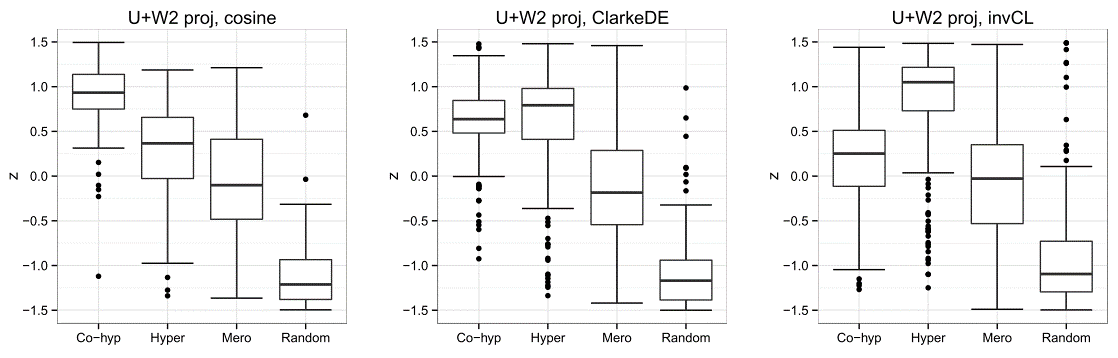
\includegraphics[width=1.\linewidth]{images/std_distrib_invCL_post_feature_selection.png}
  \caption{Standardised distribution of $cosine$, $ClarkeDE$, $invCL$ score across relations in \textit{U+W2} VSM, after feature selection \citep{roller2014inclusive}.}
  \label{fig:std_invCL_boxplot_500dim}
\end{figure}
The unsupervised measures were tested on the lower dimensional \textit{U+W2} vector space using the BLESS dataset.  We reproduced the figure from \citep{roller2014inclusive} in Figure~\ref{fig:std_invCL_boxplot_500dim}
Using the selected dimensions, the $ClarkeDE$ and $invCL$ measures return a higher standardised score for the hypernym term.  As expected, the $cosine$ symmetric measure was unaffected by the updated vector space and assigned a higher score to co-hyponyms.  Statistically significant results were, however, only achieved by the $invCL$ measure \citep{roller2014inclusive}.

\subsection{Unsupervised Measures as Features for Supervised Learning}
\citeauthor{santus2016nine} created another supervised-unsupervised hybrid system by using the scores emitted from various unsupervised measures as input features to several classifiers.  They originally selected thirteen unsupervised measures which are designed to capture different distributional properties of the word-pair vectors.  Feature selection was carried out by systematically excluding one feature at a time and looking at the impact on the model trained on the reduced feature set in terms of the $10$-fold cross-validated $F1$ score.  Through this exercise, four unsupervised metric features were dropped, reducing the set to nine features which included:
\begin{itemize}
    \item Target-word frequency and entropy for each word in the pair (4 features);
    \item The top $N$ context frequency and entropy for each word in the pair (4 features); 
    \item A symmetric measure called $APSyn$ \citep{santus2016unsupervised} (1 feature);
\end{itemize}
 
The supervision was provided by the \textit{ROOT9} dataset, consisting of $9,600$ pairs randomly extracted from \textit{BLESS} \citep{Baroni2011}, \textit{EVALution} \citep{santus2015evalution}, and \textit{Lenci/Benotto} \citep{benotto2015distributional}.  The word-pairs included verbs, nouns and adjective and spanned three semantic relations: co-hyponymy, hypernymy, random.  The vector space model was built from the same corpora as in \citep{santus2014chasing} with the following differences: the window-based context consisted of five words on either side of the target word; \ac{PPMI} was used to weight the feature association; only words which occurred in the joint corpus a minimum of 1,000 times were considered.  This last decision had some ramifications when the authors wanted to test their solution on the alternative \textit{Weeds} dataset \citep{weeds2014learning} since no vectors were available for several words in that dataset.

The authors performed a  battery of experiments.  The best-performing classifier was a multi-class random forest model, trained to detect whether a given word-pair is bound by co-hyponymy, hypernymy or is entirely unrelated.  With $10$-fold cross validation, an $F1$ class average of 0.907 was recorded.  Several baselines which included the use of alternative classifiers such as logistic regression, or different feature sets (cosine similarity measure, randomly initialised numbers between 0 and 1) recorded much inferior results (0.572 and 0.334 respectively), which supported the case that the random forest setup was especially effective.  

However, the result was not replicated when the same random forest model was evaluated on the \textit{Weeds} dataset \citep{weeds2014learning}.  Specifically, it struggled to correctly classify word-pairs featuring hypernymy, co-hyponymy and other relations extracted from WordNet \citep{Miller1995}.  This is not a coincidence: the \textit{Weeds} dataset was designed to eliminate the repetition of words in both the hyponym and hypernym word-pair slot.  Indeed, each word will feature at most twice: once as a hyponym and one other time as a hypernym.  This reduces the impact of hypernym memorisation \citep{levy2015supervised} since a classifier will not be exposed to enough examples of common hypernyms to provoke overfitting.  Similar lower results when evaluating on \textit{Weeds} were observed in other work \citep{shwartz2017siege}.

To test how sensitive their model is overfitting to prototypical hypernyms, \citeauthor{santus2016nine} devised a simple experiment which was replicated with the same outcome in other work \citep{shwartz2017siege}.  False hypernym pairs were generated by linking a hyponym with another word’s hypernym.  The \textit{ROOT9} classifier was evaluated on a dataset consisting of 3,200 switched hypernyms and the results reflected the severity of the problem:  up to 100\% of the hypernyms were falsely classified as hypernyms, if they also featured in the training set associated with one of its actual hyponyms.  \citeauthor{santus2016nine} mitigated this problem by enriching the random pair negative examples in the training set with switched hypernym word-pairs.  Although the $F1$ score plummeted by seven percentage points on the $10$-fold cross-validated test, only 546 random pairs were falsely classified as hypernyms.

In the next section, we will introduce word embeddings, a neural model driven mechanism to learn latent, low-dimensional vector representation of words which were used to provide features for other supervised solutions.

\section{Word Embeddings}
\subsection{Embeddings Overview}
To be included...
\subsection{Supervision with Word Embeddings} \label{supervised_embeddings}
The dense, low-dimensional word representations created with word embeddings methods make ideal features with which to train supervised classifiers.  \citep{shwartz2017siege} mounted a large, comparative experiment to study how well word embeddings features can help distinguish hypernymy from other semantic relations.  They experiment with pre-trained embeddings of various dimensionality, created by three models: word2vec skip-gram \citep{mikolov2013distributed}; GloVe \citep{pennington2014glove}; trained on dependency contexts \citep{levy2014dependency}.  For each embeddings space, the authors combined the term and candidate hypernym vectors using \textit{concat}enation \citep{baroni2012entailment} and \textit{diff}erence \citep{roller2014inclusive} vector operations.  The combined embeddings features were fed into two logistic classifiers, regularised with $L1$ and $L2$ terms.

\citeauthor{shwartz2017siege} train their supervised classifiers on the same four datasets upon which they tested an assortment of unsupervised measures, discussed in section \ref{shwartz_unsupervised}.  The datasets were split randomly and lexically, the latter following \citeauthor{levy2015supervised} recommendation to avoid lexical memorisation \citep{levy2015supervised}.  The scores were measured using \ac{AP} calculated on the top 100 most confidently predicted hypernyms ($AP@100$).

The classifiers’ performance on the randomly-split datasets is close to perfect ($1.0 \leq AP@100 \geq 0.873$) on all datasets with vector concatenation of GloVe embeddings driving the best results.  Similar to \citeauthor{levy2015supervised} findings, the high scores are influenced by \say{lexical memorisation} to some degree.  Indeed, the worst result was observed when evaluating the \textit{Weeds} \citep{weeds2014learning} dataset, which is designed to avoid memorisation by featuring each of the words $(x, y)$ exactly once in the $x$ or $y$ position.  However, hypernymy was still correctly predicted 87.3\% of the time on the Weeds dataset, suggesting the classifiers were able to home in on some features in the word vectors beyond the word itself.

Furthermore, \citeauthor{shwartz2017siege} discover that the overall performance of the classifiers is not overly penalised when the classifiers were trained on the lexically-split dataset.  They blame \citeauthor{levy2015supervised} poor results on lexically-split data on a shortage of training pairs, seeing that they sacrificed 50\% of the pairs to obtain a perfectly split dataset.  On their part, \citeauthor{shwartz2017siege} discarded only around 30\% of the pairs.  Thus, the authors are less sceptical about supervised methods’ ability to abstract away from words than \citeauthor{levy2015supervised} who posit that supervision merely recalls often-seen “prototypical” hypernyms in the training set.

Having said that, \citeauthor{shwartz2017siege} do not dispute that supervised methods are not able to capture relational features which tie the hyponym and hypernym words together.  The authors manipulated the dataset to introduce false random hypernyms by allocating true hypernyms to unrelated words as previously done in \citep{santus2016nine, levy2015supervised}.  The results, this time, paint a bleaker picture whereby the best supervised model drops 42 points to 0.575 $AP@100$ score.  However, unsupervised methods were unaffected by the same random hypernym dataset and actually improve by a small fraction.  The experiment highlights the robustness of unsupervised methods backed as they are by linguistic hypotheses and agnostic to lexical patterns embedded in a training set.  The authors suggest that unsupervised methods should be considered even when training data is available. Moreover, they can mutually benefit supervised methods as we have seen in previous work \citep{roller2014inclusive, santus2016nine}.

\subsection{Integrating Word Embeddings with Path-based Approach}
Recall \textsc{HypeNET} from section \ref{HypeNet}, the system created in \citep{shwartz2016path} which generates generalised hypernymy dependency paths using an \ac{LSTM} \citep{hochreiter1997long} encoder. The authors improved their path-only model by concatenating term and candidate hypernym word embeddings to either side of the averaged path vector.  The word vectors were furnished by GloVe pre-trained embeddings trained on a Wikipedia corpus \citep{pennington2014glove}.

To create the dataset, they followed \citep{Snow2004} by extracting directly related positive and negative instance from a variety of knowledge resources.  The latter included WordNet \citep{Miller1995} and YAGO \citep{suchanek2007yago}.  Since the solution employed dependency paths, only word-pairs that jointly occurred in the Wikipedia corpus, and which were connected by at least two unique paths were selected.

Similar to \citep{levy2015supervised}, \citeauthor{shwartz2016path} split their dataset both randomly and on a lexical basis.  The model trained on embeddings and path-based features yielded improved results compared to the path-based model and various supervised models constructed in the manner described in \ref{supervised_embeddings}.  The integrated model scored a 0.7 $F1$ score on the lexically-split dataset, marking a 6.1\% and 9.9\% improvement on the path-based and best supervised classifier respectively.  A 0.90 $F1$ score was attained on the randomly-split data by the integrated model -  a more marked improvement of 18.4\% and 20.8\% on the path-based and best supervised classifier respectively.  In all mentioned cases, the integrated model's superiority was statistically significant at a confidence level of 99\% according to the paired \textit{t-test}. 

In the next section, we will review a new family of supervised learning algorithms.  These algorithms learn a transformation matrix which projects the hyponym vector to a vector close to its hypernyminimising
the mean squared error or binary cross entropy objective function.  Such models enable hypernyms to be \textit{generated} rather than merely identified and are particularly amenable to the challenge outlined in SemEval-2018 Task 9 shared task \citep{camacho2018semeval}.

\section{Hypernym Discovery and Projection Learning}
In \citep{camacho2017we}, the author lamented the fact that no effort was spared to devise methods to identify hypernyms but notes that hypernym identification is limited in usefulness.  More effort needs to be poured in hypernym discovery, whereby a system generates hypernyms from the input features of a word-pair.  

However, most of the methods we reviewed so far were designed to map an input word-pair to an unsupervised score or supervised class label.  The supervised model returns the most probable semantic class a word-pair belongs to, according to the model’s learned parameters.  The unsupervised score is harder to interpret.  A higher score suggests a higher degree of hypernymy but a threshold needs to be found, across which a word-pair can be considered to be linked by hypernymy.  

Unsupervised methods can be used in a hypernym discovery setting as they were in the SemEval-2018 Task 9 unsupervised baselines created for the task \citep{camacho2018semeval}.  Given some bounded vocabulary, different words can be plugged in the measures’ $y$-word slot and the words returning the highest score returned as potential hypernyms.  On the other hand, the supervised methods we have seen so far – possibly with the exception of \citep{Snow2004} – were shown to suffer from lexical memorisation which would “discover” the most prominent hypernyms encountered in a training set irrespective of the query term.    Discovering hypernyms from Hearst patterns is viable \citep{hearst1992automatic, wu2012probase, Snow2004} but the assumption that hypernyms and hyponyms have to co-occur in the sentence will limit these methods’ coverage.  

\begin{figure}[ht!] 
  \centering
  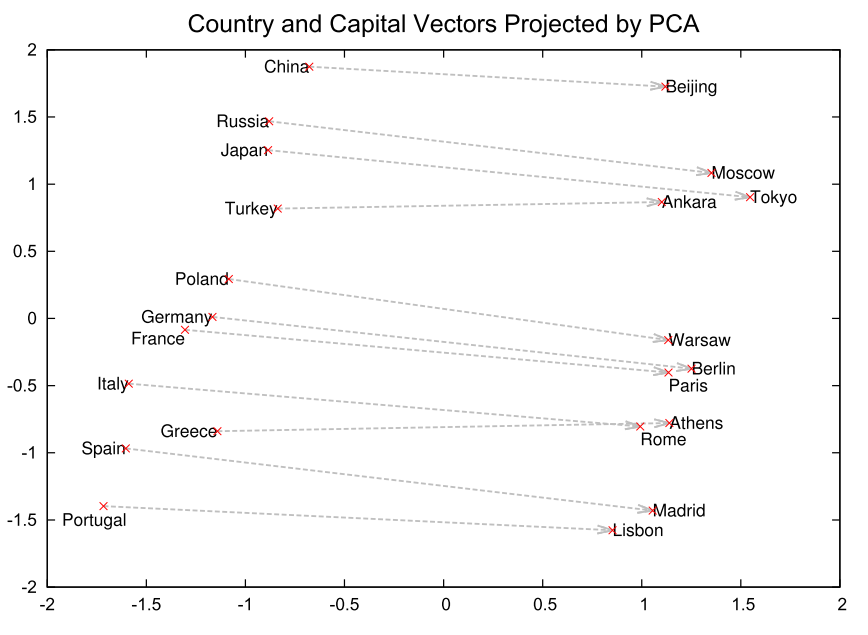
\includegraphics[width=1.\linewidth]{images/mikolov_semantic_regularity.png}
  \caption{Linear regularities between country and capital city retained in word embeddings from \citep{mikolov2013distributed}.}
  \label{fig:mikolov_capital_cities}
\end{figure}

\subsection{Early Work}
Word embeddings do not only represent word with continuous low-dimensional vectors but also retain semantic regularities in the vector space.  Figure~\ref{fig:mikolov_capital_cities} is reproduced from \citep{mikolov2013distributed} and illustrates the linear relationship between countries and their capital cities, after the distributional space is reduced to two dimensions using \ac{PCA}.  \ac{PCA} is a dimension reduction technique that reprojects the original features onto orthogonal axes (referred to as \textit{eigenvectors}) while still trying to capture most of the variance in the data.

Embedding offsets somewhat capture the relationship between words.  \citep{Fu2014} observe that the same phenomenon also applies to hyponyms and their hypernyms: vector offsets between hyponyms and hypernyms in similar domains were found to be similar.  Thus, the hyponym vector can be projected to its hypernym by applying a linear transformation.  Since it is unfeasible to calculate a separate linear projection for every hyponym, the authors propose learning an approximate projection $\bm{\Phi}$ which brings the dot product $\bm{\Phi} \cdot \bm{x}$ as close as possible to its hypernym $\bm{y}$.  Finding the optimal $\bm{\Phi}$ for our feature vector $\bm{x}$ requires the vector equivalent of scalar linear regression and can be approximated using the \ac{MSE} objective function:
\[\hat{\bm{\Phi}} = \argmin_{\bm{\Phi}} \frac{1}{N} \sum_{(x,y)} \Vert \bm{\Phi}\cdot\bm{x} - \bm {y} \Vert^2 \]

Stochastic gradient descent was the optimizer used to converge to the best solution for $\bm{\Phi}$ which returns the lowest average error over the training set.  The input word $\bm{x}$’s vector dimensions and $\bm{\Phi}$'s dimensions must be compatible to allow the dot product to be evaluated.  In general, $\bm{x}, \bm{y} \in \mathbb{R}^{d \times 1}$ represent the embeddings where $d$ is the embeddings dimensionality (typically between 50 and 300).  Therefore, the projection square matrix is $\bm{\Phi} \in \mathbb{R}^{d \times d}$ and the projected hypernym is $\bm{\Phi} \cdot \bm{x} \in \mathbb{R}^{d \times 1}$, which has the same dimensionality as the embeddings.  This allows it to be subtracted from the hypernym embedding $\bm{y}$ and the $L2$ norm can be computed on the vector offset to determine the distance between the estimated and the actual hypernym.  

The embedding vector space is too wide to expect any hyponym and its hypernym to have similar offsets.  In fact, $\bm{y}_{dog} - \bm{x}_{police\_dog} \approx \bm{y}_{fish} - \bm{x}_{tropical\_fish}$ but $\bm{y}_{dog} - \bm{x}_{police\_dog} \not \approx \bm{y}_{actor} - \bm{x}_{clown}$ \citep{Fu2014}.  \citeauthor{Fu2014} find that embeddings vector offsets make suitable dimensions for a clustering algorithm and they adapt the standard \ac{MSE} equation to a piecewise linear projection function:
\[\hat{\bm{\Phi}_k} = \argmin_{\bm{\Phi}_k} \frac{1}{N_k} \sum_{(x,y) \in C_k} \Vert \bm{\Phi}_k \cdot \bm{x} - \bm {y} \Vert^2 \]
The clusters are learnt using the unsupervised $k$-means algorithm, where the optimal $k$ is tuned on a validation set.  The clustering algorithm is fitted on the (hypernym – hyponym) vector offset which partitions the training data into distinct, semantically-related clusters.  Subsequently, a projection transformation matrix is learnt for the samples in each cluster.  Unseen pairs are first allocated to a cluster by transforming the vector offsets of their hypernym and hyponym representation using the $k$-means model fitted on the training data.  Hypernyms are discovered by first applying the learnt transformation matrix on the hyponym vector through the dot product operation, choosing the appropriate projection matrix based on the cluster assigned to the testing pair.  The closest neighbours to the estimated hypernym in the embedding space can then be found by cosine similarity or by dot-product if the vectors are first normalised to unit-length.

\citeauthor{Fu2014} do not cast the task as hypernym discovery, choosing instead to evaluate their solution within the familiar hypernym identification frame.  They focused on the Chinese language, starting from learning word embeddings from a 780-million word Chinese encyclopaedia corpus (Baidubaike) using word2vec’s skip-gram strategy \citep{mikolov2013efficient}, obtaining $560,000$ word embeddings.  $15,247$ training word-pairs were collated from \textit{CilinE}, a Chinese semantic thesaurus.  The evaluation set was sourced from the embeddings corpus and manually labelled by two annotators, ultimately settling on $1,391$ word-pairs which achieved an inter-annotator agreement score of 0.96.  One fifth of the evaluation set was retained as a development set.

The authors classify a word-pair $(x, y)$ as hypernymy as follows. They first assign a cluster to a word-pair, based on the cluster centroid which is closest by Euclidean distance to the vector offset $y - x$.  A positive match is found either: i) if the \ac{MSE} between the estimated hypernym and actual hypernym does not exceed a set threshold; or ii) if the estimated hypernym is close to another word $z$ such that is $z$ is a hyponym of the hypernym $y$, thus linking $x$ and $y$ through transitivity.

The $k$ number of clusters was tuned using the aforementioned development set, with the best performance recorded with 20 clusters and corresponding linear transformation matrices.  \citeauthor{Fu2014} measured performance using precision, recall and $F1$ score and their embeddings-based solution scored 80.54, 67.99 and 73.74 respectively.  A classification error analysis revealed that linear transformations could not be learnt if cosine similarity between the hyponym and hypernym in the embedding space exceeded 0.9038.  The authors reflect that having several training examples of this type could alleviate the problem.

\subsection{Negative Sampling} \label{Ustalov}
The family of algorithms which learn a transformation matrix via stochastic gradient descent was coined \textit{projection learning} by 
\citeauthor{ustalov2017negative} who introduced the notion of negative sampling to \citeauthor{Fu2014}'s method \citep{ustalov2017negative}.  They observed that, normally, datasets used to train supervised models include both positive and negative examples.  Since a word’s nearest neighbours in the embedding space can be linked to the word via several semantic relations, the projection learning model must be shown examples of non-hypernymy to nudge the linear projection matrix away from projecting hyponyms to their synonyms, co-hyponyms, random words or back to the original hyponym.  However, unlike the binary cross-entropy objective function used in logistic classification, an \ac{MSE} loss function cannot deal with negative examples in the training set.

\citeauthor{ustalov2017negative} devise a number of regularisation terms which can be optionally added to the original \ac{MSE} objective function and minimised together.  The regularisation term is weighted by a constant $\lambda$ hyper-parameter which allows the experiment-taker to control how much importance is allocated to the regularisation term:
\[\hat{\bm{\Phi}} = \argmin_{\bm{\Phi}} \frac{1}{\vert P \vert} \sum_{(x,y) \in P} \Vert \bm{\Phi}\cdot\bm{x} - \bm {y} \Vert^2 + \lambda R\]

The regularisation terms reflect two main linguistic constraints.  In the first instance, the authors want to reinforce the asymmetric nature of hypernymy.  Applying the projection matrix back on to $\bm{\Phi} \cdot \bm{x}$ should not generate a vector similar to the original hyponym vector x and is penalised accordingly.  This option is ideal if no negative examples are available since we only require the hyponym itself to manage the regularisation term.
\[R = \frac{1}{\vert P \vert} \sum_{(x,) \in P} \big( \hat{\bm{y}} \bm{\Phi} \cdot \bm{x} \big)^2  \]
In the equation above, the regularisation term $R$ become larger the more similar the re-projected vector and the hyponym vector are. 

The second regularisation variant \citeauthor{ustalov2017negative} propose corrects the transformation matrix from projecting the hyponym to a semantically-related word that is not hypernymy.  The authors refer to this regularisation class as \say{neighbour regularisation} and use synonyms of hyponyms as the set of negative examples $N$, but other semantic relations are also valid as are randomly unrelated words.
\[R = \frac{1}{\vert N \vert} \sum_{(x,z) \in N} \big( \hat{\bm{y}} \bm{\Phi} \cdot \bm{z} \big)^2\]
Variants of the regularisation terms that are not reliant on re-projection were also included in the study.  The authors mounted experiments in the Russian and English language although we will focus mostly on the latter since English is the language of interest in this research project.

\citeauthor{ustalov2017negative} followed the methodology we have explored so far when working on the Russian language by converting a corpus into a vector space model, in this case opting for skip-gram word embeddings using the word2vec algorithm \citep{mikolov2013efficient}.  However, they departed from convention when working on the English language, by using 300-dimensional word embeddings pre-trained on the 100-billion token Google News corpus \citep{mikolov2013efficient}.  The projection learning model with additional regularisation terms was trained on a combination of four commonly-used datasets: \textit{EVALution} \citep{santus2015evalution}; \textit{BLESS} \citep{Baroni2011}; \textit{ROOT09} \citep{santus2016nine}; and \textit{K\&H+N} \citep{necsulescu2015reading}.  Each dataset features word-pairs linked together by an assortment of semantic relations.  The word-pairs linked by hypernymy constitute the positive pairs while the other semantic relations were used to provide \say{neighbour regularisation} example terms.  

The authors followed previous work \citep{levy2015supervised, shwartz2017siege, santus2016nine, roller2014inclusive} by performing a lexical split on the Russian dataset, but do not follow suit with the combined English dataset.  Since pre-trained word-embeddings are used, words which don’t have corresponding embeddings were discarded.  The dataset was ultimately split to 4,374 training pairs, 1,540 testing pairs and 1,483 validation pairs \footnote{These counts differ from the numbers cited in \citep{ustalov2017negative}.  However, the authors privately acknowledged a mistake in their paper to us: they included words that were dropped due to having no corresponding embeddings, which reduced the dataset size.}.  Synonyms and co-hyponyms were available for 1,314 terms, with each hyponym having between 1 and 39 relata.  The clustering mechanism used in \citep{Fu2014} is followed in \citeauthor{ustalov2017negative}’s work whereby the optimal number of clusters is tuned on the validation test, the training examples are allocated to their respective cluster based on the vector offset $y - x$, and a projection matrix is learned piecewise for the word-pairs in each cluster.  The best results on the combined English datasets were observed with 25 clusters.

In contrast to \citep{Fu2014}, \citeauthor{ustalov2017negative} framed the problem as a hypernym discovery task and evaluated the results accordingly.  Instead of precision, recall and $F1$ scores, they opted for $hit@l$ (similar to $precision@k$) and \ac{AUC}.  The authors chose to evaluate at $l=(1, 5, 10)$.  While $hit@l$ simply returns the average ratio of correct results in the first $l$-slots, \ac{AUC} also considers the rank of the predicted hypernyms.  The results they achieved showed that the regularisation terms added to the \ac{MSE} loss function improved the scores achieved on all metrics and across the English and Russian datasets, irrespective of the number of clusters trained.  

However, the improvement margin between the scores achieved with and without regularisation (controlling for the number of clusters), is slight.  Statistical significance (or otherwise) was not reported in their paper but the percentage improvement between the baseline score and highest score achieved by any one of the regularisation options is, on average, 1.3\%.  Regularisation terms had a greater impact on the single cluster model, where a 13\% improvement on the baseline was recorded.  However, in general, much better results were achieved with the 25 cluster model which is consistent with \citeauthor{Fu2014}'s findings.

\subsection{Sense Awareness and Domain Clustering}
\citeauthor{espinosa2016supervised} contribute several developments to the projection learning research with their \textsc{TaxoEmbed} framework \citep{espinosa2016supervised}:
\begin{enumerate}
    \item They used a large sense-annotated repository to source the hypernym word-pairs; 
    \item They complemented the training set by unifying term-hypernyms pairs extracted from Open Information Extract (OIE) knowledge-bases;
    \item The embeddings are trained on a sense-annotated corpus which learns word-sense vectors;
    \item The clustering strategy is distinguished from previous attempts by partitioning the training space according to domain of knowledge rather than vector offset;
    \item They expand the partitioned training sets by exploiting the multiple lexicalisation words available for every concept;
\end{enumerate}

The sense inventory is provided by \textit{BabelNet} \citep{navigli2012babelnet}, a large multi-lingual, semantic repository encompassing both concepts and named entities and which is largely populated from knowledge embedded in Wikipedia and WordNet.  Like WordNet, words are organised in synsets containing one or more lexicalisations of words with the same meaning.  For instance the word (or lexicalisation) \textit{mole} is featured in 18 synsets among which:
\begin{itemize}
    \item The concept \say{spy who works against enemy espionage} sense (bn:00023221n) which includes the lexicalisations \textit{counterspy}, \textit{deep cover agent};
    \item The concept \say{molecular weight} sense (bn:00041297n) which includes the words \textit{mol}, \textit{gram molecule} as alternative lexicalisations;
    \item The named entity \say{Mole} (bn:03210051n) in the \textit{The Wind in the Willows} character sense;
\end{itemize}
The latest BabelNet 4.0 contains approximately 16 million synsets which are connected through semantic relations such as hypernymy, co-hyponymy, synonymy and so forth, extracted from WordNet.  Therefore, a hypernym of \textit{mole} in the espionage sense is \textit{spy} while in the \textit{molecular weight} sense, a hypernym is \textit{metric weight unit}.

\citeauthor{espinosa2016supervised} first mined 5.3 million hyponymy-hypernym synset pairs from the Wikidata branch of BabelNet and a further 1.35 million relations from various OIE knowledge bases.  The terms harvested from the knowledge bases are unaligned since they originated from different sources.  To resolve this problem, they leveraged the \textbf{KB-Unify} framework \citep{delli2015knowledge} to allocate the word-pairs into their corresponding BabelNet synsets and merge equivalent relations across disparate knowledge bases together.

Traditional word embeddings vectors represent words in surface-level form but the training pairs are expressed at the word-sense level.  For the sense embeddings, the authors employ \textsc{SensEmbed} \citep{iacobacci2015sensembed}, which represents word-senses in latent, continuous vector space.  The vectors were built by training word2vec \citep{mikolov2013efficient} on a sense-disambiguated version of Wikipedia, with each vector representing the concatenation of the word-form together with its corresponding BabelNet synset (ex: mole\_bn:03210051n).  In doing so, \textsc{SensEmbed} avoids the conflation of ambiguous homonyms into a single vector which results in a richer semantic space.   

The training word-pair clusters were not induced as in \citep{Fu2014, ustalov2017negative}; instead the content sections which separate Wikipedia’s featured articles \footnote{https://en.wikipedia.org/wiki/Wikipedia:Featured\_articles} by topic were used as cluster labels.  The authors reported 34 content sections (as at date of publishing), examples of which include \textit{Biology}, \textit{Food and Drink}, and \textit{Media}.  Each content section featured an average of 128 sample articles, chosen by Wikipedia as exemplary articles with respect to the high standards they met.  Training set terms were associated with a domain by creating a representative vector of each domain and then choosing the domain mostly associated with a synset via a lexical similarity metric.

The task was accomplished by leveraging \textsc{Nasari} \citep{camacho2016nasari} – a multilingual vector representation which represents words and their BabelNet senses in a joint semantic space.  Lexical domain vectors having words as dimensions, weighted by lexical specificity \citep{camacho2016nasari} were constructed from the concatenation of high-quality articles chosen by Wikipedia as representative of each domain.  Lexical specificity is a metric which returns the most representative words for a given text based on the hypergeometric distribution and is found to be superior to the conventional \ac{tf-idf} which was previously used to determine word relevance in a document \citep{camacho2016nasari}.  The similarity between each domain lexical vector and a training synset’s corresponding \textsc{Nasari} lexical vector was computed using Weighted Overlap (WO), a function that compares two vectors in terms of the rank of their overlapping dimensions.  The term synset was added to the domain whose vector returned the maximum WO score.

After domain clustering, the authors were able to augment the training set further by expanding the hyponym and hypernym sense concepts into their respective lexicalisations.  For example, new training pairs could be created by adding  \textit{counterspy\_bn:00023221n} and \textit{deep\_cover\_agent\_bn:00023221n} to the hyponym \textit{mole\_bn:00023221n}.  Similarly,  \textit{undercover\_agent\_bn:00073685n} was added to the  \textit{spy\_bn:00073685n} hypernym sense.  In this way, the original Wikidata and aligned OIE datasets were increased three and eleven-fold respectively.  

At this stage, a transformation matrix can be learned for each domain cluster by minimising \ac{MSE} similar to \citep{Fu2014}.  Like \citeauthor{ustalov2017negative}, \citeauthor{espinosa2016supervised} framed the task as a hypernym discovery problem.  They held out 250 test terms form each domain.  Finding potential hypernyms is more involved than \citep{ustalov2017negative} since the terms are expressed as BabelNet concepts rather than words.  Each test term concept is expanded to its lexicalisation vectors and the vocabulary words closest (by cosine similarity) to the dot-product of the cluster transformation matrix and lexicalisation vectors are found.  Each lexicalisation’s candidate hypernyms are ranked such that a condensed list of hypernyms can be returned for the lexicalisations’ sense concept.  Performance is evaluated on \ac{MAP}, \ac{MRR} and $precision@k$ .

In general, performance increased with training set size and having a mix of Wikidata and complementary \textbf{KB-U} training pairs.   Some domains such as \textit{Education}, benefitted particularly from a sizeable set of \textbf{KB-U} training pairs since the latter featured a large amount of \textit{is-a} knowledge about North American education institutions, which boosted the coverage of educational concepts.

Performance was also found to be influenced by the domain.  The best \ac{MAP} and \ac{MRR} scores were registered in the \textit{Biology} domain at 0.84 and 0.83 respectively.  The authors speculate that this was primarily due to the formal hierarchical division of flora and fauna, in itself an area of study that has been around for hundreds of years.  Lexical memorisation \citep{levy2015supervised} may have also had a part to play with the transformation matrix learning to project hyponym terms to prototypical hypernyms such as \textit{taxon}, \textit{vertebrate} and so on.   On the other hand, the \textit{Health} and \textit{Warfare} domains scored lowest with a maximum \ac{MAP} of 0.11 and 0.05 respectively; the \textit{Health} domain did not particularly benefit from an increase of training samples.  The authors do not provide reasons behind these (comparatively) poor results but one does suspect the opposite of the prototypical hypernym effect with a wide distribution of possible hypernyms that reduces any lexical memorisation advantage.

Finally, \citeauthor{espinosa2016supervised} demonstrate empirically the advantage of a piecewise projection matrix trained independently on a cluster of semantically related word-sense pairs.  When they introduced a large number of random pairs (hence, pairs which were not formally allocated a domain) to the various domains, the results were uniformly bad.  From all reported data, this results is a \ac{MAP} between 0 and 0.06, with the only outlier being the \textit{Biology} domain where a model trained on domain-unspecific sense pairs still managed a 0.81 \ac{MAP}.  Once again, this was attributed to the lexical memorisation phenomenon. 

\subsection{Joint-Learning of Clusters and Projection Matrices} \label{yamane_in_review}
In contrast to the projection learning research we have examined so far, \citeauthor{yamane2016distributional} do not rely on the $L2$ norm between the projected hypernym vector and the gold-standard vector to measure how well hypernymy is being estimated.  Similarity, instead, is computed using the dot product of the unit-normalised estimated hypernym vector and actual hypernym embeddings.  The authors were directly motivated by the approach used in word2vec training \citep{mikolov2013efficient} whereby the similarity between the target word vector and context word vector was also computed by the dot product operation.  The similarity score is fed to a sigmoid function which estimates the probability that the projected hypernym vector is a good approximation of the word’s actual hypernym vector.  

The authors propose additional changes to the hypernym generation architecture.  The clusters are not allocated prior to training but are jointly learnt with the cluster parameters \citep{yamane2016distributional}.  Their model starts by creating a single cluster defined by the cluster parameters $\bm{\Phi}_1$,  a randomly-initialised projection square matrix, and a cluster scalar bias term $b_1$ initialised to 0.  The model computes the similarity $s$ with respect to a cluster $c$ for each word-pair $(x,y)$ in the training set according to the equation: 
\[s_c = \sigma\big( (\bm{\Phi}_c \cdot \bm{x}) \cdot \bm{y} + b_c \big)\]
If the maximum similarity for the training sample $(x,y)$ across all clusters does not exceed a threshold $\lambda$, the model assumes that none of the current clusters can adequately absorb the word-pair.  Thus, new cluster parameters are initialised and the word-pair is allocated to the new cluster.  Otherwise, if the maximum threshold is exceeded, the word-pair is allocated to the cluster yielding the highest similarity score. 

After a word-pair is mapped to a cluster, this cluster’s parameters are updated for the projection matrix and similarity measure.  Inspired by the negative sampling in word2vec, \citeauthor{yamane2016distributional} choose $m$ negative hypernyms $z$ of $x$ to discourage the model from projecting false hypernyms. The model’s ability to deal with negative examples is another novelty that distinguishes \citeauthor{yamane2016distributional}'s work from the pioneering effort of \citep{Fu2014}. The model learns the parameters by minimising the binary cross-entropy objective function across all $k$ clusters:
\[J(\bm{\Phi}; b) = \sum_{c=1}^{k} \sum_{(x,y) \in P_c} \Big[ -log \big(s_c(\bm{x}, \bm{y}) \big) - \sum_{i=1}^{m} log \big(1 - s_c(\bm{x}, \bm{z}_i) \big) \Big]\]
The authors experiment with Japanese and English, but we focus on English since it is aligned with our research.  Like \citep{ustalov2017negative}, the authors use readily-available English resources.  The word embeddings are pre-trained on the 100-billion word Google News corpus \citep{mikolov2013efficient} and the training, test and evaluation sets are the same \citep{baroni2012entailment} used in their experiments of supervised learning on lexical entailment.

The \citep{baroni2012entailment} dataset was partially derived from \textit{BLESS} \citep{Baroni2011} and included random pairs.  However, \citeauthor{yamane2016distributional} fed their model only positive examples since negative samples were generated on the fly during training.  Words having the highest cosine similarity to the hyponym vector $\bm{x}$ in the embeddings space were selected as negative samples.  The authors settled on a single negative example for every positive pair $(m=1)$.  The dataset was split such that 70\% of pairs were used for training, 25\% used for evaluation and 5\% used to tune the hyper-parameters such as $m$ negative samples and $\lambda$ similarity threshold.

Stochastic gradient descent was optimised by Adam \citep{kingma2014adam} where $\beta_1$, $\beta_2$ and the initial learning rate hyper-parameters were set according to the recommendations outlined in their paper.  Evaluation was performed on two levels.  Firstly, the joint-learning model with inner product similarity was compared to the “pipeline” model in \citep{Fu2014} which hard-clustered the terms prior to training and then learn piecewise projection matrices by minimising the mean square error objective function.  Secondly, the impact of multiple clusters on the performance was examined, but only on the Japanese dataset.  The English hypernymy dataset was roughly 6.5\% the size of its Japanese counterpart and probably not diversified enough for the model to learn more than two clusters. 

Unlike \citeauthor{Fu2014, espinosa2016supervised}, the test terms are not already allocated to a cluster prior to evaluation.  To determine the likelihood that a word $w$, taken from the embeddings space vocabulary, is a hypernym of a test term $x$:
\begin{itemize}
    \item Each cluster’s model forward-pass algorithm is invoked with inputs $\bm{x}$ and $\bm{w}$ to return the hypernym similarity between the two vectors;
    \item The similarity score for the candidate hypernym $w$ is the maximum score returned from all the cluster models;
    \item The words are ranked in descending order of maximum similarity score and the top $N$ candidates are emitted for evaluation;
\end{itemize}

\begin{table*}\centering
    \begin{tabular}{@{}rrrrrcrrrr@{}} \toprule
    & \multicolumn{4}{c}{\textbf{Development Set}} & \phantom{a} & \multicolumn{4}{c}{\textbf{Test Set}} \\ 
    & \multicolumn{2}{c}{Japanese} & \multicolumn{2}{c}{English} && \multicolumn{2}{c}{Japanese} & \multicolumn{2}{c}{English} \\ 
    %\midrule
    \cmidrule{2-5} \cmidrule{7-10}
    & \textit{Pipeline} & \textit{Joint} & \textit{Pipeline} & \textit{Joint} && \textit{Pipeline} & \textit{Joint} & \textit{Pipeline} & \textit{Joint} \\ \midrule
    \# Clusters & 1 & 1 & 1 & 1 && 5 & 19 & 1 & 2 \\
    \ac{MRR} & 0.215 & \textbf{0.279} & 0.321 & \textbf{0.343} && 0.193 & \textbf{0.349} & 0.280 & \textbf{0.339} \\
    \bottomrule
    \end{tabular}
    \caption{\ac{MRR} comparison between pipeline and joint models and cluster size \citep{yamane2016distributional}.}\label{tab:yamane_results}
\end{table*}

The authors focused on the joint-learning model’s ability to generate highly-ranked, correct hypernyms and opted for \ac{MRR} as evaluation metric.  We merge the results reported in the authors' paper in a single table, Table~\ref{tab:yamane_results} from \citet{yamane2016distributional}.

The \ac{MRR} yielded by the inner product model, proposed by \citep{yamane2016distributional} exceeds the “pipeline” model \citep{Fu2014} on both the Japanese and English development sets, controlling for a single projection matrix to focus on the effect of the objective function.  

Furthermore, \ac{MRR} was found to increase with the number of clusters and the joint-model showed the ability to learn higher-quality clusters than the pipeline model was able to induce from the $y-x$ vector offsets using the hard-clustering approach.  \citeauthor{yamane2016distributional}'s model was only able to learn two clusters over the English dataset, but this was enough to improve the \ac{MRR} score by 21\% over the best-tuned “pipeline” model.  When evaluating Japanese hypernymy, the authors controlled the number of learnt clusters by tuning the $\lambda$ threshold hyper-parameter.  \ac{MRR} increased with the number of clusters, hitting a peak (0.368) at 19 clusters after which performance gently decreased.  They also found that validation \ac{MRR} was unstable during the initial training epochs during which new clusters were created, and then proceeded to stabilise as the model settled on the optimal number of clusters.

\citeauthor{yamane2016distributional} do not examine the lexical memorisation bias especially in the English context where it was shown to be pronounced \citep{levy2015supervised, shwartz2017siege}.  Splitting the dataset on a lexical basis rather than on a random basis would have lowered the risk of learning prototypical hypernyms but, judging on previous studies, would have probably had an adverse impact on the model’s performance.

\subsection{CRIM Modifications to Yamane et al.} \label{CRIM}
The work submitted to Semeval-2018 Task 9 competition \citep{camacho2018semeval} by researchers affiliated with the \ac{CRIM} achieved the best scores in the English subtasks from all submitted solutions.  Several resources are provided by the task organisers including gold-standard datasets for each subtask and an extensive vocabulary to limit the candidate term search space.  The CRIM solution featured two components:
\begin{itemize}
    \item A supervised projection learning method using the inner-product vector operation to measure similarity between the projected and the actual hypernym embeddings, as introduced in \citep{yamane2016distributional};
    \item An unsupervised method which matches co-occurring hyponyms and hypernyms via the standard Hearst patterns \citep{hearst1992automatic} but which also leverages cosine similarity of their embeddings representation to assign a higher weight to words that are also distributionally similar to each other;
\end{itemize}

To increase recall in the unsupervised mode, the authors follow \citep{Snow2004, ritter2009anyway} and search for conjunction patterns in the corpus to harvest co-hyponyms $q'=(q'_1,\ldots,q'_k )$ of a given term query $q$.  The occurrence frequency of each co-hyponym $q'_i$ is recorded and a co-hyponym is scored by multiplying its occurrence frequency by the cosine similarity of $(q, q'_i)$.  The co-hyponyms are ranked by their score and the highest-scoring words are retained.  The harvested co-hyponyms are used to augment the mined hypernyms of $q$ since the coverage of the original hypernym is extended.  The hypernyms are ranked using the same method employed for the co-hyponym ranking.

In this section we will focus on \citeauthor{bernier2018crim}'s extensions to the inner-product similarity method introduced by \citep{yamane2016distributional}.  The authors’ most prominent deviation is opting out of clustering the training pairs as was done in the literature so far \citep{Fu2014, espinosa2016supervised, yamane2016distributional}.  Instead, they propose a trainable fixed tensor consisting of $k$ projection matrices $\bm{\Phi}_i \in \mathbb{R}^{d \times d}$ for $i \in \{1,\ldots,k\}$ where $d$ is the dimensionality of the embeddings.  Each linear projection matrix is applied to the hyponym embeddings to produce $k$ hypernyms projections $\bm{P} \in \mathbb{R}^{k \times d}$.  The vectors are normalised to unit length, and the similarity between each projected hypernym vector and the ground-truth positive or negative hypernym in the dataset is computed using the dot product.  The linear combination of $k$ similarity scores and $k+1$ weights (an intercept term is included) is fed to a sigmoid activation function which computes the probability that the training word-pair $(x,y)$ is linked by hypernymy.  The authors reported the best results were attained when they set $k=24$.  

The similarity weights and $k$ projection matrices are learnt by minimising the binary cross-entropy cost function.  Like \citep{yamane2016distributional}, they leverage Adam \citep{kingma2014adam} to optimize the gradient descent but override the recommended hyper-parameters by setting $\beta_1 = \beta_2 = 0.9$.

Apart from learning fixed multi-projection matrices, \citeauthor{bernier2018crim} carried out additional refinements to \citep{yamane2016distributional}.  They experimented with a projection matrix initialisation strategy whereby they added random noise - drawn from a normal distribution with mean 0 and stardard deviation set as per \citep{glorot2010understanding} - to an identity matrix.  Ablation experiments executed by the authors showed that this initialisation strategy helped the model achieve better results than when the projection matrices were just randomly initialised.

The authors also found that their model benefitted from a higher positive to negative sample ratio than an equal positive to negative ratio advocated in \citep{yamane2016distributional} where every training gradient update is based on a single positive and negative example.  The best results were observed when ten random negative hypernym samples were drawn from the vocabulary for every positive hypernm in the training set.  Moreover, down-sampling high frequency hypernyms had a positive effect when tuning their model on the development set but later tests revealed that scores would have been higher if the model was trained on all datapoints.  Notwithstanding, their official results were based on down-sampled runs.

\citep{yamane2016distributional} eschew regularisation entirely or do not report provisions taken in their publication.  \citeauthor{bernier2018crim} are aware of their model’s tendency to over-fit and add dropout to the word embeddings as well as the hypernym projection vector.  Furthermore, they use gradient clipping to avoid large gradient updates to the model in the back-propagation step, especially during the first training epochs and also employ early stopping to halt training once no improvement is observed on the validation set for a consecutive number of epochs.

The largest performance boost in the CRIM model was observed when the embeddings were fine-tuned.  The embeddings were initially pre-trained on each input corpus corresponding to the various sub-tasks, using the word2vec skipgram algorithm with negative sampling \citep{mikolov2013efficient}.  Prior to training the embeddings, the corpora were pre-processed such that bi-grams and tri-grams featured in the vocabulary were merged into an atomic token.  In all projection learning setups we considered so far, the embeddings weights are frozen and do not contribute to minimising the loss functions.  Training the embeddings specialises them for the task at hand, but could also result in the embeddings “forgetting” the semantic represenation learnt from the pre-training on the corpus, vastly limiting their usefulness \citep{howard2018universal}.  The authors do not report how the embeddings were tuned but ablation tests show that training the embeddings alongside the projection matrices and sigmoid layer weights improved the \ac{MAP} score by 45\% to 143\%, depending on which other features they excised from their model.

\begin{table*}\centering
    \begin{tabular}{@{}rrrrrcrrrr@{}} \toprule
    & \multicolumn{9}{c}{\textbf{General-purpose English Dataset 1A}} \\ \cmidrule{2-10} 
    & \multicolumn{4}{c}{Projection Learning} & \phantom{a} & \multicolumn{4}{c}{Hybrid} \\
    \cmidrule{2-5} \cmidrule{7-10}
    & $MRR$ & $MAP$ & $P@1$ & $P@5$ && $MRR$ & $MAP$ & $P@1$ & $P@5$ \\ \midrule
    Given Dataset & 0.349 & 0.191 & 0.288 & \textit{N/A} && 0.359 & 0.195 & 0.297 & 0.187 \\
    Augmented Dataset & 0.345 & 0.190 & 0.283 & \textit{N/A} && \textbf{0.361} & \textbf{0.198} & \textbf{0.297} & \textbf{0.190} \\
    \bottomrule
    \end{tabular}
    \caption{\ac{CRIM} results achieved using projection learning only and hybrid results on the general-purpose English dataset \citep{bernier2018crim}.}\label{tab:CRIM_results}
\end{table*}

As mandated by the shared task's  set objective \citep{camacho2018semeval}, \citep{bernier2018crim} created a model able to discover hypernyms rather than merely identify hypernymy.  To find the most likely hypernyms for a given query term $q$, the trained model's prediction function was invoked for every word in the vocabulary, and the 15 top-ranked words were emitted as likely hypernym candidates.

Like \citep{espinosa2016supervised}, \citeauthor{bernier2018crim} are aware that neural methods benefit from more training data, and tried to bolster their results by augmenting their dataset with synthetic examples.  They exploited word distributional similarity in the embeddings by finding a query’s nearest neighbour (measured by cosine similarity) in the embeddings space and considering that word a co-hyponym.  Similar to \citep{Snow2004, ritter2009anyway}, the authors assign the original query’s hypernym to the “synthetic” co-hyponym and include this as a new word-pair in the dataset.  Similarly, if two or more hypernyms share the same nearest neighbour, the latter is also considered a bona-fide hypernym, paired with the relevant hyponyms and added to the dataset.  

Amplifying the dataset had a positive effect on the results but only when combined with the unsupervised approach.  The synthetic examples had a slight detrimental effect on the projection learning supervised method.

\section{SemEval-2018 Task 9: Hypernym Discovery}
%
%Five subtasks were curated together with a corresponding corpus:
%\begin{enumerate}
%    \item English general-purpose corpus taken from the 3-billion word \textit{UMBC} corpus \citep{han2013umbc_ebiquity};
%    \item Spanish general-purpose corpus culled from a 1.8-billion-word corpus \citep{cardellino2016spanish};
%    \item Italian general-purpose corpus called \textit{itWac} extracted from various web sources within the .it domain \citep{baroni2009wacky};
%    \item Domain-specific corpus, music, in English.  A 100-million word concatenated corpus of music-related texts including music biographies from \textit{Last.fm} contained in ELMD 2.9, articles related to music from Wikipedia, and album customer reviews from Amazon \citep{oramas2016elmd};
%    \item Domain-specific corpus, medicine, in English.  130-million word corpus picked from MEDLINE, a collection of scientific publications and other academic documents;
%\end{enumerate}

We explored hypernym discovery in the context of the SemEval-2018 Task 9 shared task \citep{camacho2018semeval}.  The competition featured a revamped benchmark for representing hypernymy, extending it from the traditional binary classification task to retrieval of candidate hypernyms from a given corpus.  The organisers set out an ambitious challenge composed of five subtasks encompassing three languages.  Contestants could develop systems to find hypernyms in Spanish and Italian, besides English.  Alongside the three general-purpose corpora in English, Spanish and Italian, the organisers also provided two domain-specific, English corpora covering the medical and music domains respectively.  However, we specifically focused on the challenging general-purpose English language task, motivated by the considerable research carried out on this language and the fact that we had no prior experience in the area.

In the following sub-sections, we will describe the English data that accompanied the shared task. A description of the three information retrieval  metrics used to evaluate the results will follow. The authors included supervised and unsupervised baselines of varying sophistication against which any solution was compared; these will also be briefly mentioned.  Eleven models were submitted of which three were not accompanied by technical papers.  The submitted model which was most relevant to our work due to it obtaining the best result in the English subtasks was explored in section \ref{CRIM}.  The other submissions will be briefly reviewed in the final subsection.

\subsection{Shared Task Datasets}
Unlike previous work undertaken in the hypernym discovery and identification research areas, this challenge steered away from the dependency on Wikipedia as underlying source corpus \citep{espinosa2016supervised, shwartz2016path, shwartz2017siege} and 
standard datasets such as \textit{BLESS}, \textit{Weeds} and others for training and evaluation \citep{ustalov2017negative, yamane2016distributional, shwartz2016path}.  

Three subtasks were designed for the English language.  The first (1A), required participants to extract hypernyms from a 3-billion-word general-purpose corpus sourced from \textit{UMBC} \citep{han2013umbc_ebiquity}.  The \textit{UMBC} corpus is made up of high-quality, heterogenous paragraphs extracted from several domains.  The other two subtasks focused on texts specific to the medical and music domains.  Participants were invited to evaluate  models trained directly on the domain-specific datasets but were also encouraged to cross-evaluate models trained on general-purpose English.  Training data is often not available for highly specialised domains and such an experiment can help determine the suitability of general models to discover hypernyms from text on which the models were never trained.

Details regarding the Spanish and Italian corpora, datasets can be found in the paper \citep{camacho2018semeval}.

\subsubsection{Dataset Construction}
The construction of the dataset was subdivided in four steps:
\begin{enumerate}
    \item Creation of vocabulary;
    \item Collection and selection of input terms;
    \item Extraction of gold hypernyms;
    \item Validation and filtering of extracted hypernyms;
\end{enumerate}
All possible hypernyms were collected in one vocabulary dataset for every subtask.  Words in the vocabulary were considered on the basis of frequency in source text.  Words had to be featured five and three times for inclusion in the general-purpose and domain-specific vocabularies respectively.  $N$-grams were included up to tri-grams as long as they too exceeded the frequency thresholds.  Exceedingly general concepts with low descriptive power (ex. \textit{entity}) were semi-automatically black-listed by first compiling a list of most common hypernyms and then manually retaining the ones which still provided useful information (ex. \textit{animal}).

Candidate hyponyms (terms) also had to exceed the same frequency threshold instituted in vocabulary creation step.  Similarly, bi-grams and tri-grams were allowed.  Only terms having at least one hypernym were ultimately considered.  Terms were automatically extracted via the application of a semi-automatic two-step process.  Bearing in mind frequency, type and knowledge domain criteria, terms were automatically extracted.  Each term was normalised manually by singularising each word, capitalising proper nouns, and lower-casing concepts.  Finally, ambiguous terms and terms incorrectly mapped to a domain were removed.

For each term, all BabelNet \citep{navigli2012babelnet} synsets were first retrieved which featured the term as a lexicalisation.  The parent nodes of each synset, across all lexical references were visited.  All lexicalizations of the visited synsets as featured in BabelNet were selected, given that they also existed in the corresponding vocabulary.
After, a two-step verification process ensured the quality of the extracted hypernyms.  The first validation run was crowdsourced, delegated to proven workers from Amazon Mechanical Turk (AMT).  Each query term and candidate hypernyms was assigned to three workers who were asked to select the correct hypernyms.  Gold labels were decided on the basis of majority voting.  Then, expert human validators were first tasked to remove incorrect hypernyms and normalise correct hypernyms (ex. singularise).  In the case of the English dataset, this step was skipped and the validation job delegated to the AMT workers.  All datasets, including the English one, were once again processed by the expert validators who, in the second case, were asked to add obvious, missing hypernyms and remove mislabelled hypernyms that were neglected by the crowdsourced validators.

\subsubsection{Why is the Dataset Challenging?}
The shared task dataset is distinguishable from the standard datasets in the following ways:
\begin{itemize}
    \item Besides single words, the dataset also features bi-grams and tri-grams.  Multi-token words can be dealt by averaging the constituent word vectors or by fusing the individual words in an atomic token and considering them as a single word; 
    \item The query terms are split between common concepts and proper noun entities.  Models can be trained on concepts and entities separately or on concepts and entities in unison;
    \item The domain distribution is varied encompassing a wide range of domains.  
    \item Word senses are conflated.  Hypernyms are given for all senses of a given word.  For instance the gold-standard hypernyms for the query word \textit{fault} include \textit{fissure} and \textit{imperfection} which capture the geological and failure senses of the lexicalisation;
    \item The dataset is noisy whereby the gold standard pairs are not necessarily correct.  For instance, the given hypernyms for \textit{Campo San Polo} (Venetian square) include \textit{topological manifold} and \textit{hausdorff space} which are two mathematical concepts that are unrelated to the single \textit{public square} sense of the word.  Models will therefore have to confront training pairs which will actually penalise their performance.  This was confirmed to us in private correspondence with \citeauthor{camacho2018semeval} who also intimated that a revamped version of the challenge is in the works.
\end{itemize}

\subsubsection{English General-purpose Dataset Metrics}
\begin{table*}\centering
    \begin{tabular}{@{}lrrrr@{}} \toprule
    & \multicolumn{4}{c}{\textbf{General-purpose English Dataset 1A}} \\ \cmidrule{2-5}
    & \textit{Term Count} & \textit{Word-pairs} & \shortstack[r]{\textit{Intra-set}\\\textit{Uniq. Hypers.}} & \shortstack[r]{\textit{Inter-set}\\\textit{Uniq. Hypers.}} \\ \midrule
    Training & 1,500 & 11,779 & 4,233 & 2,480 \\
    Test & 1,500 & 7,048 & 3,076 & 1,323 \\ \midrule
    \textbf{Total} & 3,000 & 18,827 & 5,556 & 5,556 \\
    \bottomrule
    \end{tabular}
    \caption{English, general-purpose dataset metrics.}\label{tab:semeval_english_dataset_metrics}
\end{table*}
As can be seen from Table~\ref{tab:semeval_english_dataset_metrics}, term words are often linked to several hypernyms.  Although the term words are lexically split in the training and test sets - that is, the same term does not appear in both datasets - the same cannot be said of the hypernyms.  Indeed, from 3,076 distinct hypernyms in the test set, 1,753 also feature in the $y$-slot of one or more word-pairs in the training set.  The lexical memorisation phenomenon studied in \citep{levy2015supervised} was also observed in one of the shared task's submitted work \citep{bernier2018crim}.  In the supervised context, creating lexically separated datasets would likely inhibit prototypical hypernyms from being "discovered" but would also reduce the training set appreciably, thus limiting the potential of a supervised model.  Unsupervised techniques are agnostic to lexical split or lack thereof \citep{shwartz2017siege}.

Not included in Table~\ref{tab:semeval_english_dataset_metrics}, is a small validation set made up of 200 word-pairs (50 terms) which was also provided by the organisers in addition to the training and test sets.  To constrain the hypernym search space, a 218,753 $n$-gram ($n \leq 3$) vocabulary of possible hypernym terms was supplied.  

\subsection{Evaluation Metrics}
Similar to other work \citep{espinosa2016supervised, ustalov2017negative} focused on hypernym discovery, the shared task organisers borrowed a set of metrics normally used to evaluate information retrieval solutions \citep{bian2008finding}.  For the top 15 hypernyms extracted for each input concept in the relevant subtask, the
following information retrieval measures were utilised:
\begin{enumerate}
    \item Mean Average Precision.  $AP(\cdot)$ (average precision) returns the percentage of correct hypernyms for a particular query word from a bounded list of retrieved words.  Averaging $AP$ over all query words gives us the mean average precision: 
    \[MAP = \frac{1}{\vert Q \vert} \sum_{q \in Q} AP(q)\]
    \item Mean Reciprocal Rank. For each query term, this metric finds the rank of the first correct hypernym from a list of retrieved words ($rank_i$); calculates the reciprocal of this value and finally computes the arithmetic mean of the reciprocal rank for all queries:
    \[MRR = \frac{1}{\vert Q \vert} \sum_{i=1}^{\vert Q \vert} \frac{1}{rank_i}\]
    \item Precision$@k$. Return the average precision at specific cut-off points $k$ where $k \in \{1, 3, 5, 15\}$ as defined in \citep{camacho2018semeval}
\end{enumerate}
An analysis of the evaluation code provided by \citeauthor{camacho2018semeval}, reveals that the authors also consider the number of gold hypernyms associated with a term when evaluating the hypernyms discovered for that query.  They ignore the words that occupy a rank $> n_{gold}$, where $n_{gold}$ is the number of gold hypernyms provided for a particular query term.  For instance, \textit{monetary unit} is the only gold hypernym for \textit{dirham}; in that case the metric functions will ignore all hypernyms ranked $2^{nd}$ to $15^{th}$ and only evaluate the top-ranked hypernym retrieved for \textit{dirham}.

\subsection{Baselines}
Participating systems were compared against research-grounded supervised and unsupervised baselines.  Two supervised baselines were developed.  The first was a na\"ve occurrence-based metric, which simply emitted the 15 most frequent hypernyms featured in the training set and was called \ac{MFH}.  The second baseline was a single-cluster version of \textsc{TaxoEmbed} \citep{espinosa2016supervised}, eschewing the domain adaptation component of the original, referred to as \textit{vanilla Taxoembed}.

The unsupervised baselines first required pre-processing the corpus and mapping it to a \ac{VSM} using a methodology similar to what was reported in several work we reviewed in this dissertation \citep{shwartz2017siege, santus2014chasing, roller2014inclusive}.  Three linguistic hypotheses (refer to Table~\ref{tab:unsupervised_measures}) were represented by a metric chosen from each respective "family". Symmetric similarity was represented by \textbf{APSyn} \citep{santus2016unsupervised}; \textbf{balAPInc} \citep{kotlerman2010directional} characterised the distributional inclusional hypothesis while informativeness was based on \textbf{SLQS} \citep{santus2014chasing}.

\begin{table*}\centering
    \begin{tabular}{@{}lrrrcrrrcrrr@{}} \toprule
    & \multicolumn{11}{c}{\textbf{General-purpose English Dataset 1A}} \\
    \cmidrule{2-12}
    & \multicolumn{3}{c}{\textbf{Concepts}} & \phantom{a} & \multicolumn{3}{c}{\textbf{Entities}} & \phantom{a} & \multicolumn{3}{c}{\textbf{Both}} \\ 
    \cmidrule{2-4} \cmidrule{6-8} \cmidrule{10-12}
    & \textit{MAP} & \textit{MRR} & \textit{p@5} && 
      \textit{MAP} & \textit{MRR} & \textit{p@5} && 
      \textit{MAP} & \textit{MRR} & \textit{p@5} \\  \midrule
    \textbf{vTE} & 0.069 & 0.160 & 0.065 && 0.192 & 0.424 & 0.179 && 0.106 & 0.238 & 0.099 \\
    \textbf{MFH} & 0.047 & 0.125 & 0.041 && 0.184 & 0.426 & 0.166 && 0.088 & 0.214 & 0.078 \\
    \textbf{APSyn} & 0.017 & 0.037 & 0.017 && 0.005 & 0.014 & 0.005 && 0.014 & 0.030 & 0.014 \\
    \textbf{balAPInc} & 0.017 & 0.039 & 0.017 && 0.005 & 0.015 & 0.004 && 0.014 & 0.032 & 0.013 \\
    \textbf{SLQS} & 0.007 & 0.017 & 0.007 && 0.004 & 0.009 & 0.003 && 0.006 & 0.015 & 0.006 \\
    \bottomrule
    \end{tabular}
    \caption{Baseline performance on the English, general-purpose dataset from \citep{camacho2018semeval}}.\label{tab:semeval_baseline}
\end{table*}

The baseline results can be viewed in Table~\ref{tab:semeval_baseline}, slightly adapted from \citep{camacho2018semeval}.  \textit{vanilla Taxoembed} (vTE) returned the best score when evaluating the English, general-purpose subtask (1A) although it was bested by \ac{MFH} in every other subtask \citep{camacho2018semeval}.  This is a manifestation of lexical memorisation and an effect of splitting the dataset randomly rather than lexically \citep{levy2014dependency}.  In general, the unsupervised baselines fared poorly despite optimising the metrics' various hyper-parameters \citep{camacho2018semeval}.  They placed last in the overall rankings in every subtask except two (Italian 1B, Spanish 1C).  However, unsupervised systems submitted by the participants, especially those based on embeddings vectors had a better showing as we see in the next section.

\subsection{Submitted Results}
\textbf{CRIM} was the projection learning/Hearst pattern hybrid proposed in \citep{bernier2018crim} which achieved the best scores in all English subtasks and which was described in section \ref{CRIM}.  Interestingly, an application of the piecewise projection-learning system originally proposed in \citep{Fu2014}, failed to deliver remarkable results \citep{qiu2018nlp_hz}.  This prompted \citeauthor{qiu2018nlp_hz} to build \textbf{NLP\_HZ}, a simpler, supervised model which leverages word2vec skip-gram embeddings \citep{mikolov2013efficient} to find a test term's closest neigbours in the training set using cosine similarity and then returning the gold-standard hypernyms of these neighbouring words as the retrieved candidates \citep{qiu2018nlp_hz}.  This solution  fared particurly well in the Spanish and Italian subtasks.

On the unsupervised front, \textbf{ADAPT} yielded superior results to the unsupervised baselines in the medical (2A) sub-task \citep{maldonado2018adapt}.  Once again skip-gram word embeddings \citep{mikolov2013efficient} were used to create word features.  The solution simply returned the 15 nearest neighbours of a query term word according to cosine similarity.  Their solution was harmed by not merging multi-token words into a single token, opting instead to represent n-grams by the mean of the words' constituent vectors.  Similarly, the system was only able to emit single word results while 82\% and 92\% of the medical and music domain input words respectively are multi-word terms.

\textbf{EXPR} is an integrated path-based and distributional model similar to \citep{shwartz2016path} but computational inefficiency stopped its developers from processing the entire corpora curtailing its potential \citep{aldine2018expr}.  Motivated by \citep{hearst1992automatic, Snow2004}, \textbf{APOLLO} also exploits lexico-syntactic patterns to link hyponyms to their hypernyms.  \citeauthor{onofrei2018apollo} reduced 44 lexico-syntactic pattern to 8 syntactic patterns,  claiming their solution is language independent albeit only evaluating it within the general-purpose English context; time constraints prevented them from testing their solution on the Spanish and English sub-tasks.

\section{Conclusion}
Although unsupervised pattern-matching methods are enjoying a revival \citep{roller2018hearst} and have been effectively used to extract hypernyms ever since Marti Hearst pioneered the field in 1992 \citep{hearst1992automatic}, we decided to focus on a family of algorithms known as \textit{projection learning} \citep{ustalov2017negative}.  The assumption is that a regular, linear relationship exists between the hyponym vector and its corresponding hypernym vector.  Machine-learning architectures were developed to learn this linear transformation matrix which can be applied to any hyponym and which should subsequently yield a vector at close proximity to its real hypernym/s.  These solutions were mainly motivated by the inadequacy of earlier supervised systems \citep{baroni2012entailment, weeds2014learning}) which compelled them to pick salient hypernyms in the given training set and subsequently associate a hypernymy relationship between any query word and these often-represented hypernyms.

Projection learning is a \textit{niche} family of algorithms for which, to our knowledge, standard APIs have not yet been developed.  We focused on four solutions whereby I was motivated to analyse whether features in one solution could be successfully adapted to another model. In the next chapter we will describe a series of experiments designed to gain a deep understanding of the projection learning algorithms and develop a critical stance towards them.  We will explore how the algorithms behave when exposed to two distinct datasets: one a combination of highly-curated datasets traditionally used to evaluate hypernymy classification algorithms \citep{Baroni2011, santus2015evalution, santus2016nine, necsulescu2015reading}; the other a larger, more diverse dataset that was partly derived automatically and partly validated by experts \citep{camacho2018semeval}.  The latter dataset was extracted from a large English corpus and was one of the resources published alongside the SemEval-2018, Task 9 shared task \citep{camacho2018semeval}.

We run experiments on each projection learning setup reviewed in the literature, to study: hard-clustered projection \citep{Fu2014}; learning clusters alongside the transformation matrices \citep{yamane2016distributional}; the effect of negative sampling \citep{ustalov2017negative}; and \ac{CRIM}’s modifications on the \citep{yamane2016distributional} model which yielded the highest score in the English general-purpose shared task \citep{bernier2018crim}.  

\citeauthor{ustalov2017negative} provided the codebase required to replicate their published results although the provided evaluation metrics are different from the metrics employed by the SemEval-2018, Task 9 organisers.  \citep{yamane2016distributional} and \citep{bernier2018crim} models were not available beyond their theoretical description at the time of experimentation so were implemented from scratch using the Keras framework \citep{chollet2015keras}.

This objective of this dissertation is to gain an understanding of projection learning models, first by pitting them against each other on the same standard dataset; and later by analysing how they behave on the actual shared task.  Of particular interest was to determine whether the models merely learn a projection matrix that transforms any query term to a prototypical hypernym, a reoccurrence of the lexical memorization phenomenon observed in supervised classification methods \citep{levy2015supervised}.
